\documentclass[letterpaper]{article}
\usepackage{uai2020}
\usepackage[margin=1in]{geometry}
\usepackage{times}

\usepackage[ruled,vlined]{algorithm2e}
\usepackage{amssymb}
\usepackage{mathtools}
\usepackage[capitalise]{cleveref}
\usepackage{tikz}
\usepackage{mathrsfs}
\usepackage[nounderscore]{syntax}
\usepackage{blkarray}
\usepackage{siunitx}
\usepackage{amsthm}
\usepackage[round]{natbib}
\usepackage[inline]{enumitem}

\newtheorem{constraint}{Constraint}
\theoremstyle{definition}
\newtheorem{definition}{Definition}
\newtheorem{example}{Example}

\renewcommand\fbox{\fcolorbox{red}{white}}

\makeatletter
\newcommand{\nosemic}{\renewcommand{\@endalgocfline}{\relax}}% Drop semi-colon ;
\newcommand{\dosemic}{\renewcommand{\@endalgocfline}{\algocf@endline}}% Reinstate semi-colon ;
\newcommand{\pushline}{\Indp}% Indent
\newcommand{\popline}{\Indm\dosemic}% Undent
\makeatother

\newcommand{\logical}[1]{{\normalfont \texttt{#1}}}
\newcommand{\variable}[1]{\texttt{\textup{#1}}}
\newcommand{\arrayd}[3]{\variable{{#1}[}{#2}\variable{]} \in {#3}}

% 1=name, 2=length, 3=type
\newcommand{\arrayt}[3]{\variable{{#3}} : \variable{{#1}[}{#2}\variable{]}}

\newcommand{\predicates}{\mathcal{P}}
\newcommand{\variables}{\mathcal{V}}
\newcommand{\constants}{\mathcal{C}}
\newcommand{\tokens}{\mathcal{T}}
\newcommand{\arities}{\mathcal{A}}
\newcommand{\maxArity}{\mathcal{M}_{\mathcal{A}}}
\newcommand{\maxNumNodes}{\mathcal{M}_{\mathcal{N}}}
\newcommand{\maxNumClauses}{\mathcal{M}_{\mathcal{C}}}

\DeclareMathOperator{\Determined}{\Delta}
\DeclareMathOperator{\Undetermined}{\Upsilon}
\DeclareMathOperator{\AlmostDetermined}{\Gamma}
\DeclareMathOperator{\getss}{\mathtt{:-}}

\Crefname{constraint}{Constraint}{Constraints}
\Crefname{clause}{Clause}{Clauses}
\creflabelformat{clause}{#2(#1)#3}

\usetikzlibrary{arrows.meta}
\relpenalty=10000
\binoppenalty=10000
\def\multiset#1#2{\ensuremath{\left(\kern-.3em\left(\genfrac{}{}{0pt}{}{#1}{#2}\right)\kern-.3em\right)}}

\title{Generating Random Logic Programs Using Constraint Programming}

\author{}

%\author{ {\bf Paulius Dilkas} \\
%School of Informatics \\
%University of Edinburgh \\
%Edinburgh, United Kingdom \\
%}

\begin{document}
\bibliographystyle{plainnat}
\maketitle

\begin{abstract}
  We present a novel approach to generating random logic programs and
  random probabilistic logic programs using constraint programming. The
  generated programs are useful in empirical testing of inference algorithms,
  random data generation, and program learning. This approach has a major
  advantage in that one can easily add additional conditions for the generated
  programs. As an example of this, we introduce a new constraint for predicate
  independence with efficient propagation and entailment algorithms, allowing
  one to generate programs that have a certain independence structure. In order
  to generate valid probabilistic logic programs, we also present a new
  constraint for negative cycle detection. Finally, we provide a combinatorial
  argument for correctness and describe how the parameters of the model affect
  the empirical difficulty of the program generation task.
\end{abstract}

\section{INTRODUCTION}

How confidently can we claim that an algorithm works well if it is only tested
on a few types of problems? Perhaps the `inferior' algorithm is actually
better in some specific circumstances. Maybe there are identifiable
types of inputs that make every algorithm default to exponential behaviour
that could be easily overcome with the right strategy. At present, most
inference algorithms for probabilistic logic programs are only evaluated on at
most four different problems: sometimes just a single network
\citep{DBLP:journals/tplp/KimmigDRCR11,DBLP:journals/corr/abs-1112-3785,DBLP:conf/iclp/KimmigCRDR08},
sometimes two
\citep{DBLP:journals/corr/abs-1009-3798,DBLP:conf/ecai/BruynoogheMKGVJR10} or
four networks \citep{DBLP:conf/ijcai/VlasselaerBKMR15} coming from a range of
areas such as social networks and citation/genetic/biological data sets. In
order to better understand the strengths and weaknesses of these algorithms,
along with real data they should also be evaluated on a range of synthetic
problems that accurately represent the potential complexities that have to be
handled by a well-designed inference algorithm. Furthermore, random logic
program generators can be useful in combination with methods that generate
random data with probabilistic logic programs \citep{DBLP:conf/soict/Dries15}
and can be used as a component of learning.

Most current approaches to generating random logic programs are restrictive,
e.g., limited to clauses with only two literals
\citep{DBLP:conf/lpnmr/NamasivayamT09}, or to clauses of the form $a \gets \neg
b$ \citep{DBLP:journals/tocl/WenWSL16}, but others are more expressive, e.g.,
defining a program only by the (maximum) number of atoms in the body and the
total number of rules \citep{DBLP:conf/iclp/ZhaoL03}. We introduce a way to
generate random logic programs using a constraint solver such as Choco
\citep{choco}. The same model can generate both probabilistic programs directly
in the syntax of ProbLog \citep{DBLP:conf/ijcai/RaedtKT07} as well as
non-probabilistic Prolog programs. For generated probabilistic programs to be
valid, we use a custom constraint to detect negative cycles (as described in
\cref{sec:cycles}). A major advantage of our constraint-based approach is that
one can easily add additional constraints to the model. To demonstrate that, in
\cref{sec:independence} we present a custom constraint with propagation and
entailment algorithms that can ensure predicate independence.
\cref{sec:counting} also presents a combinatorial argument for correctness,
where we produce combinatorial expressions that count the number of programs
that the model should produce for various parameter values. Finally,
\cref{sec:experiments} shows how the model scales when tasked with producing
more complicated programs and identifies the relationships between parameter
values and the empirical hardness of the program generation task.
 % TODO (Fazl): % Could you provide a motivating example? It % might be useful to engage readers.

% TODO (Vaishak):
Overall, [main] contributions are concerned purely with logic programming-based
languages and frameworks, which capture a major fragment of statistical
relational learning \citep{DBLP:series/synthesis/2016Raedt}.
However, since probabilistic logic programming [languages] are closely related
to other [endeavours] in machine learning, including (imperative) probabilistic
programming (e.g., see discussions in \citep{DBLP:journals/ml/RaedtK15}), our
results [may] provide the [footing] to explore broader questiosn on generating
and testing programs/algorithms in machine learning.

\section{PRELIMINARIES}

The basic primitives of logic programs are \emph{constants}, \emph{(logic)
  variables}, and \emph{predicates}. Each predicate has an \emph{arity} that
defines the number of terms that it can applied to. A \emph{term} is either a
variable or a constant, and an \emph{atom} is a predicate of arity $n$ applied
to $n$ terms. A \emph{formula} is a grammatically-valid expression that connects
atoms using conjunction ($\land$), disjunction ($\lor$), and negation ($\neg$).
A \emph{clause} is a pair of a \emph{head} (which is an atom) and a \emph{body}
(which is a formula). A \emph{(logic) program} is a multiset of clauses. Given a
program $\mathscr{P}$, a \emph{subprogram} $\mathscr{R}$ of $\mathscr{P}$ is a
subset of the clauses of $\mathscr{P}$ and is denoted by $\mathscr{R} \subseteq
\mathscr{P}$.

In the world of constraint satisfaction, we also have \emph{(constraint)
  variables}, each with its own \emph{domain}, whose values are restricted using
\emph{constraints}. All constraint variables in the model are integer or set
variables, however, if an integer refers to a logical construct
(e.g., a logical variable or a constant), we will make no distinction between
the two and often use names of logical constructs to refer to the underlying
integers. We say that a constraint variable is \emph{(fully) determined} if its
domain (at the given moment in the execution) has exactly one value. We will
often use $\Box$ as a special domain value to indicate a `disabled' (i.e., fixed
and ignored) part of the model. We write $\arrayd{a}{b}{c}$ to mean that
$\variable{a}$ is an array of variables of length $b$ such that each element of
$\variable{a}$ has domain $c$. Similarly, we write $\arrayt{a}{b}{c}$ to denote
an array $\variable{a}$ of length $b$ such that each element of $\variable{a}$
has type $\variable{c}$. Finally, we assume that all arrays start with index
zero.

\subsection{PARAMETERS OF THE MODEL}

We begin defining the parameters of our model by initialising sets and lists
of the primitives used in constructing logic programs: a list of predicates
$\predicates{}$, a list of their corresponding arities $\arities{}$ (so
$|\arities{}|$ = $|\predicates{}|$), a set of variables $\variables{}$, and a
set of constants $\constants{}$. Either $\variables{}$ or $\constants{}$ can be
empty, but we assume that $|\constants{}| + |\variables{}| > 0$. Similarly, the
model supports zero-arity predicates but requires at least one predicate to have
non-zero arity. For notational convenience, we also set $\maxArity{} \coloneqq
\max \arities{}$.

We also define a measure of how complicated a body of a clause can become. As
each body is represented by a tree (see \cref{sec:bodies}), we set
$\maxNumNodes{} \ge 1$ to be the maximum number of nodes in the tree
representation of any clause. We also set $\maxNumClauses{}$ to be the maximum
number of clauses in a program. We must have that $\maxNumClauses{} \ge
|\predicates{}|$ because we require each predicate to have at least one clause
that defines it. The model supports eliminating either all cycles or just
negative cycles (see \cref{sec:cycles}) and enforcing predicate independence
(see \cref{sec:independence}), so a set of independent pairs of predicates is
another parameter. Since this model can generate probabilistic as well as
non-probabilistic programs, each clause is paired with a probability which is
randomly selected from a given multiset (i.e., our last parameter). For
generating non-probabilistic programs, one can set this list equal to $\{ 1 \}$.
Finally, we define $\tokens{} = \{ \neg, \land, \lor, \top \}$ as the set of
tokens that (together with atoms) form a clause. All decision variables of the
model can now be divided into $2 \times \maxNumClauses{}$ separate groups,
treating the body and the head of each clause separately. We say that the
variables are contained in two arrays: $\arrayt{bodies}{\maxNumClauses{}}{Body}$
and $\arrayt{heads}{\maxNumClauses{}}{Head}$. Since the order of the clauses
does not change the meaning of the program, we can also state our first
constraint:

\begin{constraint}
  Clauses are sorted.
\end{constraint}

Here and henceforth, the exact ordering is immaterial: we only impose an order
to eliminate permutation symmetries.

\section{HEADS OF CLAUSES} \label{sec:heads}

\begin{definition}
  The \emph{head} of a clause is composed of a $\variable{predicate} \in
  \predicates \cup \{ \Box \}$, and
  $\arrayd{arguments}{\maxArity{}}{\constants{} \cup \variables{}} \cup \{ \Box
  \}$.
\end{definition}

Here, we use $\Box$ to denote either a disabled clause that we choose not to use
or disabled arguments if the arity of the $\variable{predicate}$ is less than
$\maxArity{}$. The reason why we need a separate value for the latter (i.e., why
it is not enough to fix disabled arguments to a single already-existing value)
will become clear in \cref{sec:variable_symmetry}.

\begin{definition} \label{def:arity}
  The \variable{predicate}'s $\variable{arity} \in [0, \maxArity{}]$ can then be
  defined using the \variable{table} constraint as the arity of the
  $\variable{predicate}$ if $\variable{predicate} \in \predicates{}$, and zero
  otherwise.
\end{definition}

Having defined arity, we can now fix the superfluous arguments:

\begin{constraint} \label{constr:arity}
  For $i = 0, \dots, \maxArity{} - 1$,
  \[
    \variable{arguments}[i] = \Box \iff i \ge \variable{arity}.
  \]
\end{constraint}

We can also add a constraint that each predicate $\mathsf{P} \in \predicates{}$
should have at least one clause with $\mathsf{P}$ at its head:

\begin{constraint}
Let
  \[
    P = \{ h.\variable{predicate} \mid h \in \variable{heads} \}.
  \]
  Then
  \[
    \variable{nValues}(P) =
    \begin{cases}
      |\predicates{}| + 1 & \text{if } \variable{count}(\Box, P) > 0 \\
      |\predicates{}| & \text{otherwise.}
    \end{cases}
  \]
\end{constraint}
% TODO (Fazl): explain what h is.

Here, $\variable{nValues}(P)$ counts the number of unique values in $P$.

\section{BODIES OF CLAUSES} \label{sec:bodies}

As was briefly mentioned before, the body of a clause is represented by a tree.

\begin{definition}
  The \emph{body} of a clause has two parts. First, we have the
  $\arrayd{structure}{\maxNumNodes{}}{[0, \maxNumNodes{} - 1]}$ array that
  encodes the structure of the tree using the following two rules:
  $\variable{structure}[i] = i$ means that the $i$-th node is a root, and
  $\variable{structure}[i] = j$ (for $j \ne i$) means that the $i$-th node's
  parent is node $j$. The second part is the array
  $\arrayt{values}{\maxNumNodes{}}{Node}$ such that $\variable{values}[i]$ holds
  the value of the $i$-th node.
\end{definition}

We can use the $\variable{tree}$ constraint \citep{DBLP:conf/cp/FagesL11} to
forbid cycles in the $\variable{structure}$ array and simultaneously define
$\variable{numTrees} \in \{ 1, \dots, \maxNumNodes{} \}$ to count the number of
trees. We will view the tree rooted at the zeroth node as the main tree and
restrict all other trees to single nodes. For this to work, we need to make sure
that the zeroth node is indeed a root:

\begin{constraint}
  $\variable{structure}[0] = 0$.
\end{constraint}

\begin{definition}
  For convenience, we also define $\variable{numNodes} \in \{ 1, \dots,
  \maxNumNodes{} \}$ to count the number of nodes in the main tree. We define it
  as
  \[
    \variable{numNodes} = \maxNumNodes{} - \variable{numTrees} + 1.
  \]
\end{definition}

\begin{figure}
  \centering
  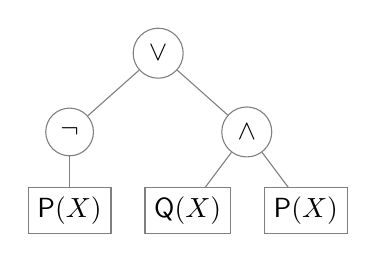
\begin{tikzpicture}
    \node[draw,circle,gray,text=black] (or) at (-0.375, 0) {$\lor$};
    \node[draw,circle,gray,text=black] (not) at (-1.5, -1) {$\neg$};
    \node[draw,circle,gray,text=black] (and) at (0.75, -1) {$\land$};
    \node[draw,gray,text=black] (P) at (-1.5, -2) {$\mathsf{P}(X)$};
    \node[draw,gray,text=black] (Q) at (0, -2) {$\mathsf{Q}(X)$};
    \node[draw,gray,text=black] (R) at (1.5, -2) {$\mathsf{P}(X)$};
    \draw[gray] (or) -- (not);
    \draw[gray] (or) -- (and);
    \draw[gray] (not) -- (P);
    \draw[gray] (and) -- (Q);
    \draw[gray] (and) -- (R);
  \end{tikzpicture}
  \caption{A tree representation of the formula from \cref{example:formula}}
  \label{fig:example_tree}
\end{figure}

\begin{example} \label{example:formula}
  Let $\maxNumNodes{} = 8$. Then
  \[
    \neg\mathsf{P}(X) \lor (\mathsf{Q}(X) \land \mathsf{P}(X))
  \]
  corresponds to the tree in \cref{fig:example_tree} and can be encoded as:
  \begin{alignat*}{8}
    \variable{structure} &= [0, &&0, &&0, &&1, &&2, &&2, &&6, &&7],\\
    \variable{values} &= [{\lor}, &&{\neg}, &&{\land}, \mathsf{P}(&&X), \mathsf{Q}(&&X), \mathsf{P}(&&X), &&\top, &&\top],\\
    \variable{numNodes} &= 6, && && && && && && &&\\
    \variable{numTrees} &= 3. && && && && && && &&
  \end{alignat*}
\end{example}

Here, $\top$ is the value we use for the remaining one-node trees. The
elements of the $\variable{values}$ array are nodes:

\begin{definition} \label{def:node}
  A \emph{node} has a $\variable{name} \in \tokens{} \cup \predicates{}$ and
  $\arrayd{arguments}{\maxArity{}}{\variables{} \cup \constants{} \cup \{ \Box
    \}}$. The node's $\variable{arity}$ can then be
  defined analogously to \cref{def:arity}.
\end{definition}

Furthermore, we can use \cref{constr:arity} to again disable the extra
arguments.

\begin{example}
  Let $\maxArity{} = 2$, $X \in \variables{}$, and let $\mathsf{P}$ be a
  predicate with arity 1. Then the node representing atom $\mathsf{P}(X)$ has:
  \begin{align*}
    \variable{name} &= \mathsf{P},\\
    \variable{arguments} &= [X, \Box],\\
    \variable{arity} &= 1.
  \end{align*}
\end{example}

% TODO (Fazl): the first four words sound odd. Rephrase.
It remains to constrain the forest represented by the $\variable{structure}$
array together with its $\variable{values}$ to eliminate unnecessary symmetries
and adhere to our desired format. First, we can recognise that the order of the
elements in the $\variable{structure}$ array does not matter, i.e., the
structure is only defined by how the elements link to each other, so we can add
a constraint saying that:

\begin{constraint}
  \variable{structure} is sorted.
\end{constraint}

Next, since we already have a variable that counts the number of nodes in the
main tree, we can fix the structure and the values of the remaining trees to
some constant values:

\begin{constraint}
  For $i = 1, \dots, \maxNumNodes{} - 1$, if $i \ge \variable{numNodes}$, then
  \[
    \variable{structure}[i] = i, \quad \text{and} \quad
    \variable{values}[i].\variable{name} = \top,
  \]
  else $\variable{structure}[i] < i$.
\end{constraint}

The second part of this constraint states that every node in the main tree
except the zeroth node cannot be a root and must have its parent located to
the left of itself. Next, we classify all nodes into three classes: predicate
(or empty) nodes, negation nodes, and conjunction/disjunction nodes based on the
number of children (zero, one, and two, respectively).

\begin{constraint} \label{constraint:node_types}
  For $i = 0, \dots, \maxNumNodes{} - 1$, let $C_i$ be the number of times $i$
  appears in the \variable{struture} array with index greater than $i$. Then
  \begin{align*}
    C_i = 0 &\iff \variable{values}[i].\variable{name} \in \predicates{} \cup \{ \top \},\\
    C_i = 1 &\iff \variable{values}[i].\variable{name} = \neg,\\
    C_i > 1 &\iff \variable{values}[i].\variable{name} \in \{ \land, \lor \}.
  \end{align*}
\end{constraint}

The value $\top$ serves a twofold purpose: it is used as the fixed value for
nodes outside the main tree, and, when located at the zeroth node, it can
represent a clause with no body. Thus, we can say that only root nodes can have
$\top$ as the value:

\begin{constraint}
  For $i = 0, \dots, \maxNumNodes{} - 1$,
  \[
    \variable{structure}[i] \ne i \implies
    \variable{values}[i].\variable{name} \ne \top.
  \]
\end{constraint}

Finally, we add a way to disable a clause by setting its head predicate to
$\Box$:

\begin{constraint}
  For $i = 0, \dots, \maxNumClauses{} - 1$, if
  $\variable{heads}[i].\variable{predicate} = \Box$, then
  \[
    \variable{bodies}[i].\variable{numNodes} = 1,
  \]
  and
  \[
    \variable{bodies}[i].\variable{values}[0].\variable{name} =
    \top.
  \]
\end{constraint}

\section{VARIABLE SYMMETRIES} \label{sec:variable_symmetry}

Given any clause, we can permute the variables in that clause without changing
the meaning of the clause or the entire program. Thus, we want to fix the order
of variables to eliminate unnecessary symmetries. Informally, we can say that
variable $X$ goes before variable $Y$ if the first occurrence of $X$ in either
the head or the body of the clause is before the first occurrence of $Y$. Note
that the constrains described in this section only make sense if $|\variables| >
1$. Also note that all definitions and constraints here are on a per-clause
basis.

\begin{definition}
  Let $N = \maxArity{} \times (\maxNumNodes{} + 1)$, and let
  $\variable{terms}[N] \in \constants{} \cup \variables{} \cup \{ \Box
  \}$ be a flattened array of all arguments in a particular clause.

  Then we can use a channeling constraint to define
  $\variable{occ}[|\constants{}| + |\variables{}| + 1]$ as an array of subsets
  of $\{ 0, \dots, N-1 \}$ such that for all $i = 0, \dots, N - 1$, and $t \in
  \constants{} \cup \variables{} \cup \{ \Box \}$,
  \[
    i \in \variable{occ}[t] \quad \iff \quad
    \variable{terms}[i] = t
  \]
\end{definition}

Next, we introduce an array that, for each variable, holds the position of its
first occurrence:

\begin{definition}
  Let $\arrayd{intros}{|\variables{}|}{\{ 0, \dots, N \}}$ be such that
  for $v \in \variables{}$,
  \[
    \variable{intros}[v] = \begin{cases}
      1 + \min \variable{occ}[v] & \text{if }
      \variable{occ}[v] \ne \emptyset\\
      0 & \text{otherwise.}
    \end{cases}
  \]
\end{definition}

Here, a value of zero means that the variable does not occur in the clause. The
reason why we want to use specifically zero for this will become clear with
\cref{constraint:diffbutzero}. Because of this choice, the definition of
$\variable{intros}$ shifts all indices by one. Lastly, we add the constraint
that eliminates variable symmetries:

\begin{constraint}
  $\variable{intros}$ are sorted.
\end{constraint}

In other words, we constrain the model so that the variable listed first in
whatever order $\variables{}$ is presented in has to occur first in our
representation of a clause.

\begin{example} \label{example:sibling}
  Let $\constants{} = \emptyset$, $\variables{} = \{ X, Y, Z \}$, $\maxArity{} =
  2$, $\maxNumNodes{} = 3$, and consider the clause
  \[
    \mathsf{sibling}(X, Y) \gets \mathsf{parent}(X, Z) \land
    \mathsf{parent}(Y, Z).
  \]
  Then
  \begin{align*}
    \variable{terms} &= [X, Y, \Box, \Box, X, Z, Y, Z], \\
    \variable{occ} &= [\{ 0, 4 \}, \{ 1, 6 \}, \{ 5, 7 \}, \{ 2, 3 \}], \\
    \variable{intros} &= [0, 1, 5],
  \end{align*}
  where the $\Box$'s correspond to the conjunction node.
\end{example}

\subsection{REDUNDANT CONSTRAINTS}

We add a number of redundant constraints to make search more efficient. First,
we can formally state that the positions occupied by different terms must be
different:

\begin{constraint} \label{constraint:all_diff}
  For $u \ne v \in \constants{} \cup \variables{} \cup \{ \Box \}$,
  \[
    \variable{occ}[u] \cap \variable{occ}[v] = \emptyset.
  \]
\end{constraint}

The reason why we used zero to represent an unused variable is so that we could
efficiently rephrase \cref{constraint:all_diff} for the $\variable{intros}$
array:

\begin{constraint} \label{constraint:diffbutzero}
  $\variable{allDifferentExcept0}(\variable{intros})$.
\end{constraint}

We can also add another link between $\variable{intros}$ and $\variable{occ}$
that essentially says that the smallest element of a set is an element of the
set:

\begin{constraint}
  For $v \in \variables{}$,
  \[
    \variable{intros}[v] \ne 0 \quad \iff \quad
    \variable{intros}[v] - 1 \in \variable{occ}[v].
  \]
\end{constraint}


Finally, we define an auxiliary set variable to act as a set of possible values
that $\variable{intros}$ can take:

\begin{definition}
  Let $\variable{potentials} \subseteq \{ 0, \dots, N \}$ be such that for $v
  \in \variables{}$, $\variable{intros}[v] \in \variable{potentials}$.
\end{definition}

Using this new variable, we can add a constraint saying that non-predicate nodes
in the tree representation of a clause cannot have variables as arguments:

\begin{constraint} \label{constraint:potentialIntroductions}
  For $i = 0, \dots, \maxNumNodes{} - 1$, let
  \[
    S = \{ \maxArity{} \times (i + 1) + j + 1 \mid j = 0, \dots, \maxArity{} - 1
    \}.
  \]
  If $\variable{values}[i].\variable{name} \not\in \predicates{}$, then
  $\variable{potentials} \cap S = \emptyset$.
\end{constraint}

\section{COUNTING PROGRAMS} \label{sec:counting}

In order to demonstrate the correctness of the model and explain it in more
detail, in this section we are going to derive combinatorial expressions for
counting the number of programs with up to $\maxNumClauses{}$ clauses and up to
$\maxNumNodes{}$ nodes per clause, and arbitrary $\predicates{}$,
$\arities{}$, $\variables{}$, and $\constants{}$. To simplify the task, we only
consider clauses without probabilities and disable (negative) cycle elimination.
It was experimentally confirmed that the model agrees with the combinatorial
formula from this section in 985 different scenarios. The \emph{total arity} of
a body of a clause is the sum total of arities of all predicates in the body.
% TODO (Vaishak, last sentence): move to footnote and add "Since the [details] of
% this empirical investigation are not crucial to the thrust of this paper, we
% will [detail] this in an extendedd technical report."

We will first consider clauses with gaps, i.e., without taking variables and
constants into account. Let $T(n, a)$ denote the number of possible clause
bodies with $n$ nodes and total arity $a$. Then $T(1, a)$ is the number of
predicates in $\predicates{}$ with arity $a$, and the following recursive
definition can be applied for $n > 1$:
\begin{align*}
  T(n, a) = T(n-1, a) + 2&\sum_{\substack{c_1 + \dots + c_k = n - 1,\\
      2 \le k \le \frac{a}{\min \arities{}},\\
  c_i \ge 1 \text{ for all } i}}\\
  &\sum_{\substack{d_1 + \dots + d_k = a,\\
  d_i \ge \min \arities{} \text{ for all } i}} \prod_{i=1}^k T(c_i, d_i).
\end{align*}
The first term here represents negation, i.e., negating a formula consumes
one node but otherwise leaves the task unchanged. If the first operation is not
negation, then it must be either conjunction or disjunction (hence the
coefficient `2'). In the first sum, $k$ represents the number of children of the
root node, and each $c_i$ is the number of nodes dedicated to child $i$. Thus,
the first sum iterates over all possible ways to partition the remaining $n-1$
nodes. Similarly, the second sum considers every possible way to partition the
total arity $a$ across the $k$ children nodes.

We can then count the number of possible clause bodies with total arity $a$ (and
any number of nodes) as
\[
  C(a) = \begin{cases}
    1 & \text{if } a = 0\\
    \sum_{n=1}^{\maxNumNodes{}} T(n, a) & \text{otherwise.}
  \end{cases}
\]
Here, the empty clause is considered separately.

The number of ways to select $n$ terms is
\begin{align*}
  P(n) = |\constants{}|^n + &\sum_{\substack{1 \le k \le |\variables{}|, \\ 0 =
      s_0 < s_1 < \dots < s_k < s_{k+1} = n+1}}\\
  &\prod_{i=0}^k (|\constants{}| + i)^{s_{i+1} - s_i - 1}.
\end{align*}
The first term is the number of ways select $n$ constants. The parameter $k$ is
the number of variables used in the clause, and $s_1, \dots, s_k$ mark the first
occurrence of each variable. For each gap between any two introductions (or
before the first introduction, or after the last introduction), we have
$s_{i+1}-s_i-1$ spaces to be filled with any of the $|\constants{}|$ constants
or any of the $i$ already-introduced variables.

Let us order the elements of $\predicates{}$, and let $a_i$ be the arity of the
$i$-th predicate. The number of programs is then:
\[
  \sum_{\substack{ \sum_{i=1}^{|\predicates{}|} h_i = n,\\
      |\predicates{}| \le n \le \maxNumClauses,\\
      h_i \ge 1 \text{ for all } i}} \prod_{i=1}^{|\predicates{}|}
  \multiset{\sum_{a=0}^{\maxArity{} \times \maxNumNodes{}} C(a) P(a+a_i)}{h_i},
\]
where
\[
  \multiset{n}{k} = \binom{n+k-1}{k}
\]
counts the number of ways to select $k$ out of $n$ items with repetition (and
without ordering). Here, we sum over all possible ways to distribute
$|\predicates{}| \le n \le \maxNumClauses{}$ clauses among $|\predicates{}|$
predicates so that each predicate gets at least one clause. For each predicate,
we can then count the number of ways to select its clauses out of all possible
clauses. The number of possible clauses can be computed by considering each
possible arity $a$, and multiplying the number of `unfinished' clauses $C(a)$ by
the number of ways to select the required $a+a_i$ terms in the body and the head
of the clause.

\section{PREDICATE INDEPENDENCE} \label{sec:independence}

In this section, we define a notion of predicate independence as a way to
constrain the probability distributions defined by the generated programs. We
also describe efficient algorithms for propagation and entailment checking.

\begin{definition}
  Let $\mathscr{P}$ be a probabilistic logic program. Its \emph{predicate
    dependency graph} is a directed graph $G_{\mathscr{P}} = (V, E)$ with the
  set of nodes $V$ consisting of all predicates in $\mathscr{P}$. For any two
  different predicates $\mathsf{P}$ and $\mathsf{Q}$, we add an edge from
  $\mathsf{P}$ to $\mathsf{Q}$ if there is a clause in $\mathscr{P}$ with
  $\mathsf{Q}$ as the head and $\mathsf{P}$ mentioned in the body. We say that
  the edge is \emph{negative} if there exists a clause with $\mathsf{Q}$ as the
  head and at least one instance of $\mathsf{P}$ at the body such that the path
  from the root to the $\mathsf{P}$ node in the tree representation of the
  clause passes through at least one negation node. Otherwise it is
  \emph{positive}. We say that $\mathscr{P}$ (or $G_{\mathscr{P}}$) has a
  \emph{negative cycle} if $G_{\mathscr{P}}$ has a cycle with at least one
  negative edge.
\end{definition}

Labelling the edges as positive/negative will be immaterial for predicate
independence, but the same graph will play a crucial role in negative cycle
detection in the next section.

\begin{definition}
  Let $\mathsf{P}$ be a predicate in a program $\mathscr{P}$. The set of
  \emph{dependencies} of $\mathsf{P}$ is the smallest set $D_{\mathsf{P}}$ such
  that $\mathsf{P} \in D_{\mathsf{P}}$, and, for every $\mathsf{Q} \in
  D_{\mathsf{P}}$, all direct predecessors of $\mathsf{Q}$ in $G_{\mathscr{P}}$
  are in $D_{\mathsf{P}}$.
\end{definition}

\begin{definition}
  Two predicates $\mathsf{P}$ and $\mathsf{Q}$ are \emph{independent} if
  $D_{\mathsf{P}} \cap D_{\mathsf{Q}} = \emptyset$.
\end{definition}

\begin{figure}
  \centering
  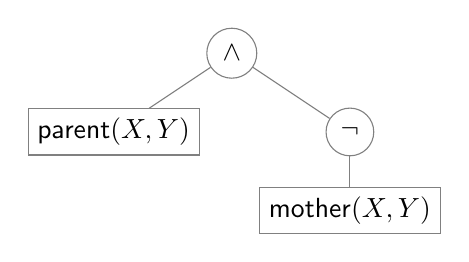
\begin{tikzpicture}
    \node[draw,circle,gray,text=black] (and) at (0, 0) {$\land$};
    \node[draw,circle,gray,text=black] (not) at (1.5, -1) {$\neg$};
    \node[draw,gray,text=black] (parent) at (-1.5, -1) {$\mathsf{parent}(X, Y)$};
    \node[draw,gray,text=black] (mother) at (1.5, -2) {$\mathsf{mother}(X, Y)$};
    \draw[gray] (and) -- (parent);
    \draw[gray] (and) -- (not);
    \draw[gray] (not) -- (mother);
  \end{tikzpicture}
  \caption{A tree representation of the body of \cref{eq:example_clause}}
  \label{fig:example_tree2}
\end{figure}
\begin{figure}
  \centering
  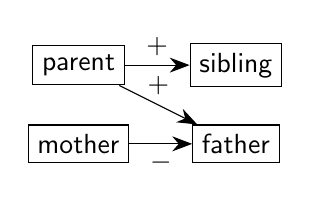
\begin{tikzpicture}
    \node[draw] (parent) at (0, 0.5) {$\mathsf{parent}$};
    \node[draw] (mother) at (0, -0.5) {$\mathsf{mother}$};
    \node[draw] (sibling) at (2, 0.5) {$\mathsf{sibling}$};
    \node[draw] (father) at (2, -0.5) {$\mathsf{father}$};
    \draw[-{Stealth[scale=1.5]}] (parent) edge node[above] {$+$} (sibling);
    \draw[-{Stealth[scale=1.5]}] (parent) edge node[above] {$+$} (father);
    \draw[-{Stealth[scale=1.5]}] (mother) edge node[below] {$-$} (father);
  \end{tikzpicture}
  \caption{The predicate dependency graph of the program in \cref{ex:program}.
    Positive edges are labelled with `$+$', and negative edges with `$-$'.}
  \label{fig:predicate_dependencies}
\end{figure}

\begin{example} \label{ex:program}
  Consider the following (fragment of a) program:
  \begin{align}
    \mathsf{sibling}(X, Y) &\gets \mathsf{parent}(X, Z) \land \mathsf{parent}(Y, Z), \nonumber \\
    \mathsf{father}(X, Y) &\gets \mathsf{parent}(X, Y) \land \neg\mathsf{mother}(X, Y) \label[clause]{eq:example_clause}
  \end{align}
  Its predicate dependency graph is in \cref{fig:predicate_dependencies}.
  Because of the negation in \cref{eq:example_clause} (as seen in
  \cref{fig:example_tree2}), the edge from $\mathsf{mother}$ to
  $\mathsf{father}$ is negative, while the other two edges are positive.

  We can now list the dependencies of each predicate:
  \begin{alignat*}{3}
    D_{\mathsf{parent}} &= \{ \mathsf{parent} \}, && D_{\mathsf{sibling}}
    &&= \{\mathsf{sibling}, \mathsf{parent} \},\\
    D_{\mathsf{mother}} &= \{ \mathsf{mother} \}, && D_{\mathsf{father}}
    &&= \{ \mathsf{father}, \mathsf{mother}, \mathsf{parent} \}.
  \end{alignat*}
  Hence, we have two pairs of independent predicates, i.e., $\mathsf{mother}$ is
  independent from $\mathsf{parent}$ and $\mathsf{sibling}$.
\end{example}

We can now add a constraint to define an adjacency matrix for the predicate
dependency graph but without positivity/negativity:

\begin{definition} \label{def:adjacency_matrix}
  An $|\predicates{}| \times |\predicates{}|$ adjacency matrix $\mathbf{A}$ with
  $\{ 0, 1 \}$ as its domain is defined by stating that $\mathbf{A}[i][j] = 0$
  if and only if, for all $k \in \{ 0, \dots, \maxNumClauses{} - 1 \}$, either
  \[
    \variable{heads}[k].\variable{predicate} \ne j
  \]
  or
  \[
    i \not\in \{a.\variable{name} \mid a \in
    \variable{bodies}[k].\variable{values} \}.
  \]
\end{definition}

Given an undetermined model, we can classify all dependencies of a predicate
$\mathsf{P}$ into three categories based on how many of the edges on the path
from the dependency to $\mathsf{P}$ are undetermined. In the case of zero, we
call the dependency \emph{determined}. In the case of one, we call it
\emph{almost determined}. Otherwise, it is \emph{undetermined}. In the context
of propagation and entailment algorithms, we define a \emph{dependency} as the
sum type:
\begin{grammar}
  <dependency> ::= $\Determined(p)$ | $\Undetermined(p)$ | $\AlmostDetermined(p,
  s, t)$
\end{grammar}
where each alternative represents a determined, undetermined, and almost
determined dependency, respectively. Here, $p \in \predicates{}$ is the name of
the predicate which is the dependency of $\mathsf{P}$, and---in the case of
$\AlmostDetermined$---$(s, t) \in \predicates{}^2$ is the one undetermined edge
in $\mathbf{A}$ that prevents the dependency from being determined. For a
dependency $d$---regardless of its exact type---we will refer to its predicate
$p$ as $d.\mathsf{predicate}$. In describing the algorithms, we will use an
underscore to replace any of $p$, $s$, $t$ in situations where the name is
unimportant.

\begin{algorithm}
  \SetKwFunction{getDependencies}{deps}
  \SetKwFunction{isDetermined}{isDetermined}
  \SetKwData{predicate}{predicate}
  \KwData{predicates $p_1$, $p_2$}
  \nosemic $D \gets \{ (d_1, d_2) \in \getDependencies{$p_1$, 1} \times \getDependencies{$p_2$, 1}$\;
  \hspace{27pt}\dosemic $\mid d_1.\predicate = d_2.\predicate \}$\;
  \lIf{$D = \emptyset$}{\Return{\textsc{true}}}
  \lIf{$\exists (\Determined \_, \Determined \_) \in D$}{\Return{\textsc{false}}}
  \Return{\textsc{undefined}}\;
  \caption{Entailment for independence}
  \label{alg:independence_entailment}
\end{algorithm}

Each entailment algorithm returns one out of three different values:
\textsc{true} if the constraint is guaranteed to hold, \textsc{false} if the
constraint is violated, and \textsc{undefined} if whether the constraint will be
satisfied or not depends on the future decisions made by the solver.
\cref{alg:independence_entailment} outlines a simple entailment algorithm for
the independence of two predicates $p_1$ and $p_2$. First, we separately
calculate all dependencies of $p_1$ and $p_2$ and look at the set $D$ of
dependencies that $p_1$ and $p_2$ have in common. If there are none, then the
predicates are clearly independent. If they have a dependency in common that is
already fully determined ($\Determined$) for both predicates, then they cannot be
independent. Otherwise, we return \textsc{undefined}.

\begin{algorithm}[h]
  \LinesNumbered
  \SetKwFunction{getDependencies}{deps}
  \SetKwFunction{fail}{fail}
  \SetKwFunction{removeValue}{removeValue}
  \SetKwData{predicate}{predicate}
  \SetKwData{source}{source}
  \SetKwData{target}{target}
  \KwData{predicates $p_1$, $p_2$; adjacency matrix $\mathbf{A}$}
  \For{$(d_1, d_2) \in \getDependencies{$p_1$, 0} \times \getDependencies{$p_2$,
      0}$ such that $d_1.\predicate = d_2.\predicate$}{
    \lIf{$d_1$ {\bf is} $\Determined(\_)$ {\bf and} $d_2$ {\bf is}
      $\Determined(\_)$}{\fail{}} \label{line:fail}
    \If{$d_1$ {\bf is} $\Determined(\_)$ {\bf and} $d_2$ {\bf is}
      $\AlmostDetermined(\_, s, t)$ {\bf or} \hspace{50pt} $d_2$ {\bf is}
      $\Determined(\_)$ {\bf and} $d_1$ {\bf is} $\AlmostDetermined(\_, s,
      t)$ \label{line:propagation_condition}}{
      $\mathbf{A}[s][t]$.\removeValue{$1$}\; \label{line:propagation_result}
    }
  }
  \caption{Propagation for independence}
  \label{alg:independence_propagation}
\end{algorithm}

Propagation algorithms have two goals: causing a contradiction (failing) in
situations where the corresponding entailment algorithm would return
\textsc{false}, and eliminating values from domains of variables that are
guaranteed to cause a contradiction. \cref{alg:independence_propagation} does
the former on \cref{line:fail}. Furthermore, for any dependency shared between
predicates $p_1$ and $p_2$, if it is determined ($\Determined$) for one
predicate and almost determined ($\AlmostDetermined$) for another, then the edge
that prevents the $\AlmostDetermined$ from becoming a $\Determined$ cannot
exist--\cref{line:propagation_condition,line:propagation_result} handle this
possibility.

\begin{algorithm}
  \SetKwData{edgeExists}{edge}
  \SetKwData{predicate}{predicate}
  \SetKwData{source}{source}
  \SetKwData{target}{target}
  \SetKwData{all}{allDependencies}
  \SetKwFunction{getDependencies}{deps}
  \SetKwProg{Fn}{Function}{:}{}
  \KwData{adjacency matrix $\mathbf{A}$}
  \Fn{\getDependencies{$p$, \all}} {
    $D \gets \{ \Determined(p) \}$\;
    \While{\logical{true}}{
      $D' \gets \emptyset$\;
      \For{$d \in D$ {\bf and} $q \in \predicates{}$}{
        $\edgeExists \gets \mathbf{A}[q][d.\predicate] = \{ 1 \}$\;
        \uIf{$\edgeExists$ {\bf and} $d$ {\bf is} $\Determined(\_)$}{
          $D' \gets D' \cup \{ \Determined(q) \}$
        }
        \uElseIf{$\edgeExists$ {\bf and} $d$ {\bf is} $\AlmostDetermined(\_, s,
          t)$}{
          $D' \gets D' \cup \{ \AlmostDetermined(q, s, t) \}$\;
        }
        \uElseIf{$|\mathbf{A}[q][d.\predicate]| > 1$ {\bf and} $d$~{\bf is}~$\Determined(r)$}{
          $D' \gets D' \cup \{ \AlmostDetermined(q, q, r) \}$\;
        }
        \ElseIf{$|\mathbf{A}[q][d.\predicate]| > 1$ {\bf and} \all}{
          $D' \gets D' \cup \{ \Undetermined(q) \}$\;
        }
      }
      \lIf{$D' = D$}{\Return{$D$}}
      $D \gets D'$\;
    }
  }
  \caption{Dependencies of a predicate}
  \label{alg:dependencies}
\end{algorithm}

The function $\getDependencies$ in \cref{alg:dependencies} calculates $D_p$ for
any predicate $p$. It has two versions: $\getDependencies(p, 1)$ returns all
dependencies, while $\getDependencies(p, 0)$ returns only determined and
almost-determined dependencies. It starts by establishing the predicate $p$
itself as a dependency and continues to add dependencies of dependencies until
the set $D$ stabilises. For each dependency $d \in D$, we look at the in-links
of $d$ in the predicate dependency graph. If the edge from some predicate $q$ to
$d.\mathsf{predicate}$ is fully determined and $d$ is determined, then $q$ is
another determined dependency of $p$. If the edge is determined but $d$ is
almost determined, then $q$ is an almost-determined dependency. The same outcome
applies if $d$ is fully determined but the edge is undetermined. Finally, if we
are interested in collecting all dependencies regardless of their status, then
$q$ is a dependency of $p$ as long as the edge from $q$ to
$d.\mathsf{predicate}$ is possible. Note that if there are multiple paths in the
dependency graph from $q$ to $p$, \cref{alg:dependencies} could include $q$ once
for each possible type ($\Determined$, $\Undetermined$, and
$\AlmostDetermined$), but
\cref{alg:independence_propagation,alg:independence_entailment} would still work
as intended.

\begin{figure}
  \centering
  \[
    \begin{blockarray}{ccccc}
      \begin{block}{c(cccc)}
        \mathsf{father} & 0 & 0 & 0 & 0 \\
        \mathsf{mother} & 1 & 0 & 0 & 0 \\
        \mathsf{parent} & 1 & \fbox{\{ 0, 1 \}} & \{ 0, 1 \} & \{ 0, 1 \} \\
        \mathsf{sibling} & 0 & 0 & 0 & 0 \\
      \end{block}
    \end{blockarray}
  \]
  \caption{The adjacency matrix defined using \cref{def:adjacency_matrix} for
    \cref{example:independence}}
  \label{fig:dependencies_matrix}
\end{figure}
\begin{figure}
  \centering
  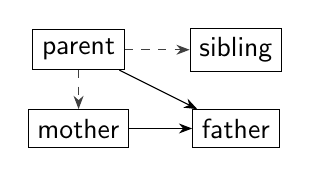
\begin{tikzpicture}
    \node[draw] (parent) at (0, 0.5) {$\mathsf{parent}$};
    \node[draw] (mother) at (0, -0.5) {$\mathsf{mother}$};
    \node[draw] (sibling) at (2, 0.5) {$\mathsf{sibling}$};
    \node[draw] (father) at (2, -0.5) {$\mathsf{father}$};
    \draw[-{Stealth}] (parent) edge (father);
    \draw[-{Stealth}] (mother) edge (father);
    \draw[-{Stealth},dashed,darkgray] (parent) edge (sibling);
    \draw[-{Stealth},dashed,darkgray] (parent) edge (mother);
  \end{tikzpicture}
  \caption{The predicate dependency graph that corresponds to
    \cref{fig:dependencies_matrix}. Dashed edges are undetermined---they may
    or may not exist.}
  \label{fig:dependencies2}
\end{figure}

\begin{example} \label{example:independence}
  Consider this partially determined (fragment of a) program:
  \begin{align*}
    \Box(X, Y) &\gets \mathsf{parent}(X, Z) \land \mathsf{parent}(Y, Z),\\
    \mathsf{father}(X, Y) &\gets \mathsf{parent}(X, Y) \land \neg\mathsf{mother}(X, Y)
  \end{align*}
  where $\Box$ indicates an unknown predicate with domain
  \[
    D_\Box = \{ \mathsf{father}, \mathsf{mother}, \mathsf{parent},
    \mathsf{sibling} \}.
  \]
  The predicate dependency graph without positivity/negativity (as defined in
  \cref{def:adjacency_matrix}) is represented in
  \cref{fig:dependencies_matrix,fig:dependencies2}.

  Suppose we have a constraint that $\mathsf{mother}$ and $\mathsf{parent}$ must
  be independent. The lists of potential dependencies for both predicates are:
  \begin{align*}
    D_{\mathsf{mother}} &= \{ \Determined(\mathsf{mother}), \AlmostDetermined(\mathsf{parent}, \mathsf{parent}, \mathsf{mother}) \}, \\
    D_{\mathsf{parent}} &= \{ \Determined(\mathsf{parent}) \}.
  \end{align*}
  An entailment check at this stage would produce \textsc{undefined}, but
  propagation replaces the boxed value in \cref{fig:dependencies_matrix} with
  zero, eliminating the potential edge from $\mathsf{parent}$ to
  $\mathsf{mother}$. This also eliminates $\mathsf{mother}$ from $D_\Box$, and,
  although some undetermined variables remain, this is enough to make
  \cref{alg:independence_entailment} return \textsc{true}.
\end{example}

\section{NEGATIVE CYCLES} \label{sec:cycles}

Having no negative cycles in the predicate dependency graph is a requirement for
probabilistic logic programming language ProbLog \citep{kimmig2009trading},
although it has been shown how the requirement can be alleviated by introducing
negative probabilities \citep{DBLP:journals/ijar/BuchmanP17}. Ideally, we would
like to design a constraint for negative cycles similar to the constraint for
independence in the previous section. However, the difficulty with creating a
propagation algorithm for negative cycles is that there seems to be no good way
to extend \cref{def:adjacency_matrix} so that the adjacency matrix captures
positivity/negativity. Thus, we settle for an entailment algorithm with no
propagation.

\begin{algorithm}
  \KwData{a program $\mathscr{P}$}
  \SetKwFunction{hasNegativeCycles}{hasNegativeCycles}
  Let $\mathscr{R} \subseteq \mathscr{P}$ be the largest subprogram of
  $\mathscr{P}$ with its $\variable{structure}$ and predicates in both body
  and head fully determined\footnotemark\;
  \If{\hasNegativeCycles($G_{\mathscr{R}}$)}{
    \Return{\textsc{false}}\;
  }
  \lIf{$\mathscr{R} = \mathscr{P}$}{\Return{\textsc{true}}}
  \Return{\textsc{undefined}}\;
  \caption{Entailment for negative cycles}
  \label{alg:negative_cycles}
\end{algorithm}
\footnotetext{The arguments (whether variables or constants) are irrelevant to
  our definition of independence.}

The algorithm takes all clauses whose structure and predicates have been fully
determined and uses them to construct a full dependency graph. In our
implementation, \texttt{hasNegativeCycles} function is just a simple extension
of the backtracking cycle detection algorithm that `travels' around the graph
following edges and checking if each vertex has already been visited or not.
Alternatively, one could assign weights to the edges (e.g., $1$ for positive
and $-\infty$ for negative edges), thus reducing our negative cycle detection
problem to what is typically known as the negative cycle detection problem in
the literature, and use an algorithm such as Bellman-Ford
\citep{shimbel1954structure}.

If the algorithm finds a negative cycle in this fully-determined part of the
program, then we must return \textsc{false}. If there was no negative cycle and
the entire program is (sufficiently) determined, then there cannot be any
negative cycles. In all other cases, it is too early to tell.

% TODO (Vaishak):
% Now we add a theorem that states that the programs generated by the algorithm,
% regardless of whether they involve negative cycles or not, are well-defined?
% That is, in the non-probabilistic case, they are satisfiable, and, in the
% probabilistic case, for both negative cycles & without, they induce programs
% that are satisfiable + well-defined measure on the set of satisfying
% assignments [proofs in the appendix?]

\section{EMPIRICAL PERFORMANCE} \label{sec:experiments}

\begin{figure}
  \centering
  % Created by tikzDevice version 0.12.3 on 2020-05-11 12:44:46
% !TEX encoding = UTF-8 Unicode
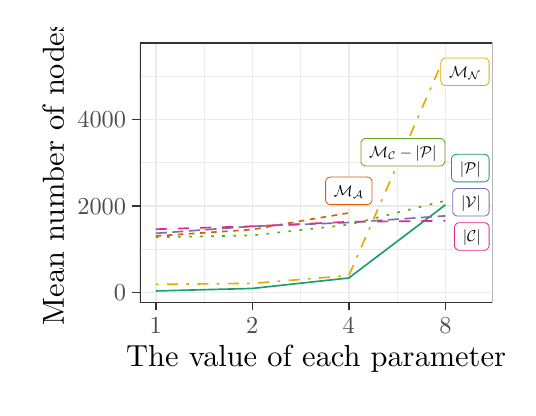
\begin{tikzpicture}[x=1pt,y=1pt]
\definecolor{fillColor}{RGB}{255,255,255}
\path[use as bounding box,fill=fillColor,fill opacity=0.00] (0,0) rectangle (173.45,130.09);
\begin{scope}
\path[clip] (  0.00,  0.00) rectangle (173.45,130.09);
\definecolor{drawColor}{RGB}{255,255,255}
\definecolor{fillColor}{RGB}{255,255,255}

\path[draw=drawColor,line width= 0.6pt,line join=round,line cap=round,fill=fillColor] (  0.00,  0.00) rectangle (173.45,130.09);
\end{scope}
\begin{scope}
\path[clip] ( 40.51, 30.69) rectangle (167.95,124.59);
\definecolor{fillColor}{RGB}{255,255,255}

\path[fill=fillColor] ( 40.51, 30.69) rectangle (167.95,124.59);
\definecolor{drawColor}{gray}{0.92}

\path[draw=drawColor,line width= 0.3pt,line join=round] ( 40.51, 50.03) --
	(167.95, 50.03);

\path[draw=drawColor,line width= 0.3pt,line join=round] ( 40.51, 81.30) --
	(167.95, 81.30);

\path[draw=drawColor,line width= 0.3pt,line join=round] ( 40.51,112.57) --
	(167.95,112.57);

\path[draw=drawColor,line width= 0.3pt,line join=round] ( 63.74, 30.69) --
	( 63.74,124.59);

\path[draw=drawColor,line width= 0.3pt,line join=round] ( 98.62, 30.69) --
	( 98.62,124.59);

\path[draw=drawColor,line width= 0.3pt,line join=round] (133.49, 30.69) --
	(133.49,124.59);

\path[draw=drawColor,line width= 0.6pt,line join=round] ( 40.51, 34.40) --
	(167.95, 34.40);

\path[draw=drawColor,line width= 0.6pt,line join=round] ( 40.51, 65.67) --
	(167.95, 65.67);

\path[draw=drawColor,line width= 0.6pt,line join=round] ( 40.51, 96.94) --
	(167.95, 96.94);

\path[draw=drawColor,line width= 0.6pt,line join=round] ( 46.30, 30.69) --
	( 46.30,124.59);

\path[draw=drawColor,line width= 0.6pt,line join=round] ( 81.18, 30.69) --
	( 81.18,124.59);

\path[draw=drawColor,line width= 0.6pt,line join=round] (116.05, 30.69) --
	(116.05,124.59);

\path[draw=drawColor,line width= 0.6pt,line join=round] (150.93, 30.69) --
	(150.93,124.59);
\definecolor{drawColor}{RGB}{27,158,119}

\path[draw=drawColor,line width= 0.6pt,line join=round] ( 46.30, 34.95) --
	( 81.18, 35.86) --
	(116.05, 39.64) --
	(150.93, 66.05);
\definecolor{drawColor}{RGB}{217,95,2}

\path[draw=drawColor,line width= 0.6pt,dash pattern=on 2pt off 2pt ,line join=round] ( 46.30, 54.81) --
	( 81.18, 57.14) --
	(101.58, 60.74) --
	(116.05, 63.15);
\definecolor{drawColor}{RGB}{117,112,179}

\path[draw=drawColor,line width= 0.6pt,dash pattern=on 4pt off 2pt ,line join=round] ( 46.30, 55.77) --
	( 81.18, 58.31) --
	(116.05, 59.68) --
	(150.93, 62.08);
\definecolor{drawColor}{RGB}{231,41,138}

\path[draw=drawColor,line width= 0.6pt,dash pattern=on 4pt off 4pt ,line join=round] ( 46.30, 57.27) --
	( 81.18, 58.33) --
	(116.05, 59.95) --
	(150.93, 60.30);
\definecolor{drawColor}{RGB}{102,166,30}

\path[draw=drawColor,line width= 0.6pt,dash pattern=on 1pt off 3pt ,line join=round] ( 46.30, 54.34) --
	( 81.18, 55.03) --
	(116.05, 58.92) --
	(150.93, 67.56);
\definecolor{drawColor}{RGB}{230,171,2}

\path[draw=drawColor,line width= 0.6pt,dash pattern=on 1pt off 3pt on 4pt off 3pt ,line join=round] ( 46.30, 37.33) --
	( 81.18, 37.69) --
	(116.05, 40.51) --
	(150.93,120.32);
\end{scope}
\begin{scope}
\path[clip] ( 40.51, 30.69) rectangle (167.95,124.59);

\path[] (158.55, 74.38) -- (150.93, 66.05);
\definecolor{drawColor}{RGB}{27,158,119}
\definecolor{fillColor}{RGB}{255,255,255}

\path[draw=drawColor,line width= 0.3pt,line join=round,line cap=round,fill=fillColor] (154.94, 74.38) --
	(164.94, 74.38) --
	(164.86, 74.38) --
	(165.15, 74.39) --
	(165.44, 74.45) --
	(165.71, 74.55) --
	(165.96, 74.70) --
	(166.19, 74.88) --
	(166.38, 75.10) --
	(166.54, 75.34) --
	(166.65, 75.61) --
	(166.72, 75.89) --
	(166.74, 76.18) --
	(166.74, 76.18) --
	(166.74, 82.51) --
	(166.74, 82.51) --
	(166.72, 82.80) --
	(166.65, 83.08) --
	(166.54, 83.35) --
	(166.38, 83.60) --
	(166.19, 83.81) --
	(165.96, 84.00) --
	(165.71, 84.14) --
	(165.44, 84.25) --
	(165.15, 84.30) --
	(164.94, 84.32) --
	(154.94, 84.32) --
	(155.16, 84.30) --
	(154.87, 84.32) --
	(154.58, 84.28) --
	(154.30, 84.20) --
	(154.04, 84.08) --
	(153.80, 83.91) --
	(153.59, 83.71) --
	(153.41, 83.48) --
	(153.28, 83.22) --
	(153.19, 82.94) --
	(153.14, 82.66) --
	(153.13, 82.51) --
	(153.13, 76.18) --
	(153.14, 76.33) --
	(153.14, 76.04) --
	(153.19, 75.75) --
	(153.28, 75.47) --
	(153.41, 75.22) --
	(153.59, 74.98) --
	(153.80, 74.78) --
	(154.04, 74.62) --
	(154.30, 74.49) --
	(154.58, 74.41) --
	(154.87, 74.38) --
	cycle;
\end{scope}
\begin{scope}
\path[clip] ( 40.51, 30.69) rectangle (167.95,124.59);
\definecolor{drawColor}{RGB}{27,158,119}

\node[text=black,anchor=base,inner sep=0pt, outer sep=0pt, scale=  0.57] at (159.94, 77.39) {$|\mathcal{P}|$};
\end{scope}
\begin{scope}
\path[clip] ( 40.51, 30.69) rectangle (167.95,124.59);
\definecolor{drawColor}{RGB}{117,112,179}
\definecolor{fillColor}{RGB}{255,255,255}

\path[draw=drawColor,line width= 0.3pt,line join=round,line cap=round,fill=fillColor] (155.41, 62.03) --
	(164.94, 62.03) --
	(164.86, 62.03) --
	(165.15, 62.04) --
	(165.44, 62.10) --
	(165.71, 62.20) --
	(165.96, 62.35) --
	(166.19, 62.53) --
	(166.38, 62.75) --
	(166.53, 63.00) --
	(166.65, 63.26) --
	(166.72, 63.55) --
	(166.74, 63.84) --
	(166.74, 63.84) --
	(166.74, 70.16) --
	(166.74, 70.16) --
	(166.72, 70.45) --
	(166.65, 70.74) --
	(166.53, 71.00) --
	(166.38, 71.25) --
	(166.19, 71.47) --
	(165.96, 71.65) --
	(165.71, 71.80) --
	(165.44, 71.90) --
	(165.15, 71.96) --
	(164.94, 71.97) --
	(155.41, 71.97) --
	(155.63, 71.96) --
	(155.34, 71.97) --
	(155.05, 71.93) --
	(154.77, 71.85) --
	(154.51, 71.73) --
	(154.27, 71.56) --
	(154.06, 71.36) --
	(153.88, 71.13) --
	(153.75, 70.87) --
	(153.65, 70.60) --
	(153.61, 70.31) --
	(153.60, 70.16) --
	(153.60, 63.84) --
	(153.61, 63.98) --
	(153.61, 63.69) --
	(153.65, 63.40) --
	(153.75, 63.13) --
	(153.88, 62.87) --
	(154.06, 62.64) --
	(154.27, 62.44) --
	(154.51, 62.27) --
	(154.77, 62.15) --
	(155.05, 62.07) --
	(155.34, 62.03) --
	cycle;
\end{scope}
\begin{scope}
\path[clip] ( 40.51, 30.69) rectangle (167.95,124.59);
\definecolor{drawColor}{RGB}{117,112,179}

\node[text=black,anchor=base,inner sep=0pt, outer sep=0pt, scale=  0.57] at (160.17, 65.04) {$|\mathcal{V}|$};
\end{scope}
\begin{scope}
\path[clip] ( 40.51, 30.69) rectangle (167.95,124.59);
\definecolor{drawColor}{RGB}{231,41,138}
\definecolor{fillColor}{RGB}{255,255,255}

\path[draw=drawColor,line width= 0.3pt,line join=round,line cap=round,fill=fillColor] (156.04, 49.68) --
	(164.94, 49.68) --
	(164.86, 49.68) --
	(165.15, 49.69) --
	(165.44, 49.75) --
	(165.71, 49.85) --
	(165.96, 50.00) --
	(166.19, 50.18) --
	(166.38, 50.40) --
	(166.54, 50.65) --
	(166.65, 50.91) --
	(166.72, 51.20) --
	(166.74, 51.49) --
	(166.74, 51.49) --
	(166.74, 57.81) --
	(166.74, 57.81) --
	(166.72, 58.10) --
	(166.65, 58.39) --
	(166.54, 58.65) --
	(166.38, 58.90) --
	(166.19, 59.12) --
	(165.96, 59.30) --
	(165.71, 59.45) --
	(165.44, 59.55) --
	(165.15, 59.61) --
	(164.94, 59.62) --
	(156.04, 59.62) --
	(156.26, 59.61) --
	(155.96, 59.62) --
	(155.68, 59.58) --
	(155.40, 59.50) --
	(155.13, 59.38) --
	(154.89, 59.21) --
	(154.69, 59.01) --
	(154.51, 58.78) --
	(154.38, 58.52) --
	(154.28, 58.25) --
	(154.24, 57.96) --
	(154.23, 57.81) --
	(154.23, 51.49) --
	(154.24, 51.63) --
	(154.24, 51.34) --
	(154.28, 51.05) --
	(154.38, 50.78) --
	(154.51, 50.52) --
	(154.69, 50.29) --
	(154.89, 50.09) --
	(155.13, 49.92) --
	(155.40, 49.80) --
	(155.68, 49.72) --
	(155.96, 49.68) --
	cycle;
\end{scope}
\begin{scope}
\path[clip] ( 40.51, 30.69) rectangle (167.95,124.59);
\definecolor{drawColor}{RGB}{231,41,138}

\node[text=black,anchor=base,inner sep=0pt, outer sep=0pt, scale=  0.57] at (160.49, 52.69) {$|\mathcal{C}|$};
\end{scope}
\begin{scope}
\path[clip] ( 40.51, 30.69) rectangle (167.95,124.59);

\path[] (139.49, 80.12) -- (150.93, 67.56);
\definecolor{drawColor}{RGB}{102,166,30}
\definecolor{fillColor}{RGB}{255,255,255}

\path[draw=drawColor,line width= 0.3pt,line join=round,line cap=round,fill=fillColor] (122.22, 80.12) --
	(148.97, 80.12) --
	(148.89, 80.12) --
	(149.18, 80.13) --
	(149.47, 80.19) --
	(149.74, 80.29) --
	(149.99, 80.44) --
	(150.22, 80.62) --
	(150.41, 80.84) --
	(150.57, 81.08) --
	(150.68, 81.35) --
	(150.75, 81.63) --
	(150.77, 81.92) --
	(150.77, 81.92) --
	(150.77, 88.25) --
	(150.77, 88.25) --
	(150.75, 88.54) --
	(150.68, 88.82) --
	(150.57, 89.09) --
	(150.41, 89.34) --
	(150.22, 89.55) --
	(149.99, 89.74) --
	(149.74, 89.88) --
	(149.47, 89.99) --
	(149.18, 90.05) --
	(148.97, 90.06) --
	(122.22, 90.06) --
	(122.44, 90.05) --
	(122.15, 90.06) --
	(121.86, 90.02) --
	(121.58, 89.94) --
	(121.32, 89.82) --
	(121.08, 89.65) --
	(120.87, 89.45) --
	(120.70, 89.22) --
	(120.56, 88.96) --
	(120.47, 88.68) --
	(120.42, 88.40) --
	(120.42, 88.25) --
	(120.42, 81.92) --
	(120.42, 82.07) --
	(120.42, 81.78) --
	(120.47, 81.49) --
	(120.56, 81.21) --
	(120.70, 80.96) --
	(120.87, 80.72) --
	(121.08, 80.52) --
	(121.32, 80.36) --
	(121.58, 80.23) --
	(121.86, 80.15) --
	(122.15, 80.12) --
	cycle;
\end{scope}
\begin{scope}
\path[clip] ( 40.51, 30.69) rectangle (167.95,124.59);
\definecolor{drawColor}{RGB}{102,166,30}

\node[text=black,anchor=base,inner sep=0pt, outer sep=0pt, scale=  0.57] at (135.59, 83.13) {$\mathcal{M}_{\mathcal{C}}-|\mathcal{P}|$};
\end{scope}
\begin{scope}
\path[clip] ( 40.51, 30.69) rectangle (167.95,124.59);
\definecolor{drawColor}{RGB}{230,171,2}
\definecolor{fillColor}{RGB}{255,255,255}

\path[draw=drawColor,line width= 0.3pt,line join=round,line cap=round,fill=fillColor] (151.08,109.18) --
	(164.94,109.18) --
	(164.86,109.18) --
	(165.15,109.19) --
	(165.44,109.25) --
	(165.71,109.36) --
	(165.96,109.50) --
	(166.19,109.68) --
	(166.38,109.90) --
	(166.54,110.15) --
	(166.65,110.42) --
	(166.72,110.70) --
	(166.74,110.99) --
	(166.74,110.99) --
	(166.74,117.32) --
	(166.74,117.32) --
	(166.72,117.61) --
	(166.65,117.89) --
	(166.54,118.16) --
	(166.38,118.40) --
	(166.19,118.62) --
	(165.96,118.80) --
	(165.71,118.95) --
	(165.44,119.05) --
	(165.15,119.11) --
	(164.94,119.12) --
	(151.08,119.12) --
	(151.30,119.11) --
	(151.01,119.12) --
	(150.72,119.09) --
	(150.44,119.01) --
	(150.18,118.88) --
	(149.94,118.72) --
	(149.73,118.51) --
	(149.56,118.28) --
	(149.42,118.02) --
	(149.33,117.75) --
	(149.28,117.46) --
	(149.28,117.32) --
	(149.28,110.99) --
	(149.28,111.13) --
	(149.28,110.84) --
	(149.33,110.56) --
	(149.42,110.28) --
	(149.56,110.02) --
	(149.73,109.79) --
	(149.94,109.59) --
	(150.18,109.42) --
	(150.44,109.30) --
	(150.72,109.22) --
	(151.01,109.18) --
	cycle;
\end{scope}
\begin{scope}
\path[clip] ( 40.51, 30.69) rectangle (167.95,124.59);
\definecolor{drawColor}{RGB}{230,171,2}

\node[text=black,anchor=base,inner sep=0pt, outer sep=0pt, scale=  0.57] at (158.01,112.19) {$\mathcal{M}_{\mathcal{N}}$};
\end{scope}
\begin{scope}
\path[clip] ( 40.51, 30.69) rectangle (167.95,124.59);
\definecolor{drawColor}{RGB}{217,95,2}
\definecolor{fillColor}{RGB}{255,255,255}

\path[draw=drawColor,line width= 0.3pt,line join=round,line cap=round,fill=fillColor] (109.46, 66.16) --
	(122.64, 66.16) --
	(122.57, 66.16) --
	(122.86, 66.17) --
	(123.15, 66.23) --
	(123.42, 66.33) --
	(123.67, 66.48) --
	(123.90, 66.66) --
	(124.09, 66.88) --
	(124.24, 67.12) --
	(124.36, 67.39) --
	(124.43, 67.67) --
	(124.45, 67.96) --
	(124.45, 67.96) --
	(124.45, 74.29) --
	(124.45, 74.29) --
	(124.43, 74.58) --
	(124.36, 74.86) --
	(124.24, 75.13) --
	(124.09, 75.38) --
	(123.90, 75.60) --
	(123.67, 75.78) --
	(123.42, 75.92) --
	(123.15, 76.03) --
	(122.86, 76.09) --
	(122.64, 76.10) --
	(109.46, 76.10) --
	(109.68, 76.09) --
	(109.39, 76.10) --
	(109.10, 76.06) --
	(108.82, 75.98) --
	(108.56, 75.86) --
	(108.32, 75.69) --
	(108.11, 75.49) --
	(107.93, 75.26) --
	(107.80, 75.00) --
	(107.71, 74.72) --
	(107.66, 74.44) --
	(107.65, 74.29) --
	(107.65, 67.96) --
	(107.66, 68.11) --
	(107.66, 67.82) --
	(107.71, 67.53) --
	(107.80, 67.26) --
	(107.93, 67.00) --
	(108.11, 66.77) --
	(108.32, 66.56) --
	(108.56, 66.40) --
	(108.82, 66.27) --
	(109.10, 66.19) --
	(109.39, 66.16) --
	cycle;
\end{scope}
\begin{scope}
\path[clip] ( 40.51, 30.69) rectangle (167.95,124.59);
\definecolor{drawColor}{RGB}{217,95,2}

\node[text=black,anchor=base,inner sep=0pt, outer sep=0pt, scale=  0.57] at (116.05, 69.17) {$\mathcal{M}_{\mathcal{A}}$};
\definecolor{drawColor}{gray}{0.20}

\path[draw=drawColor,line width= 0.6pt,line join=round,line cap=round] ( 40.51, 30.69) rectangle (167.95,124.59);
\end{scope}
\begin{scope}
\path[clip] (  0.00,  0.00) rectangle (173.45,130.09);
\definecolor{drawColor}{gray}{0.30}

\node[text=drawColor,anchor=base east,inner sep=0pt, outer sep=0pt, scale=  0.88] at ( 35.56, 31.37) {0};

\node[text=drawColor,anchor=base east,inner sep=0pt, outer sep=0pt, scale=  0.88] at ( 35.56, 62.64) {2000};

\node[text=drawColor,anchor=base east,inner sep=0pt, outer sep=0pt, scale=  0.88] at ( 35.56, 93.91) {4000};
\end{scope}
\begin{scope}
\path[clip] (  0.00,  0.00) rectangle (173.45,130.09);
\definecolor{drawColor}{gray}{0.20}

\path[draw=drawColor,line width= 0.6pt,line join=round] ( 37.76, 34.40) --
	( 40.51, 34.40);

\path[draw=drawColor,line width= 0.6pt,line join=round] ( 37.76, 65.67) --
	( 40.51, 65.67);

\path[draw=drawColor,line width= 0.6pt,line join=round] ( 37.76, 96.94) --
	( 40.51, 96.94);
\end{scope}
\begin{scope}
\path[clip] (  0.00,  0.00) rectangle (173.45,130.09);
\definecolor{drawColor}{gray}{0.20}

\path[draw=drawColor,line width= 0.6pt,line join=round] ( 46.30, 27.94) --
	( 46.30, 30.69);

\path[draw=drawColor,line width= 0.6pt,line join=round] ( 81.18, 27.94) --
	( 81.18, 30.69);

\path[draw=drawColor,line width= 0.6pt,line join=round] (116.05, 27.94) --
	(116.05, 30.69);

\path[draw=drawColor,line width= 0.6pt,line join=round] (150.93, 27.94) --
	(150.93, 30.69);
\end{scope}
\begin{scope}
\path[clip] (  0.00,  0.00) rectangle (173.45,130.09);
\definecolor{drawColor}{gray}{0.30}

\node[text=drawColor,anchor=base,inner sep=0pt, outer sep=0pt, scale=  0.88] at ( 46.30, 19.68) {1};

\node[text=drawColor,anchor=base,inner sep=0pt, outer sep=0pt, scale=  0.88] at ( 81.18, 19.68) {2};

\node[text=drawColor,anchor=base,inner sep=0pt, outer sep=0pt, scale=  0.88] at (116.05, 19.68) {4};

\node[text=drawColor,anchor=base,inner sep=0pt, outer sep=0pt, scale=  0.88] at (150.93, 19.68) {8};
\end{scope}
\begin{scope}
\path[clip] (  0.00,  0.00) rectangle (173.45,130.09);
\definecolor{drawColor}{RGB}{0,0,0}

\node[text=drawColor,anchor=base,inner sep=0pt, outer sep=0pt, scale=  1.10] at (104.23,  7.64) {The value of each parameter};
\end{scope}
\begin{scope}
\path[clip] (  0.00,  0.00) rectangle (173.45,130.09);
\definecolor{drawColor}{RGB}{0,0,0}

\node[text=drawColor,rotate= 90.00,anchor=base,inner sep=0pt, outer sep=0pt, scale=  1.10] at ( 13.08, 77.64) {Mean number of nodes};
\end{scope}
\end{tikzpicture}

  \caption{The mean number of nodes in the binary search tree for each value of
    each experimental parameter. Note that the horizontal axis is on a $\log_2$
    scale.}
  \label{fig:impact}
\end{figure}

\begin{figure*}
  \centering
  % Created by tikzDevice version 0.12.3 on 2020-01-21 13:23:35
% !TEX encoding = UTF-8 Unicode
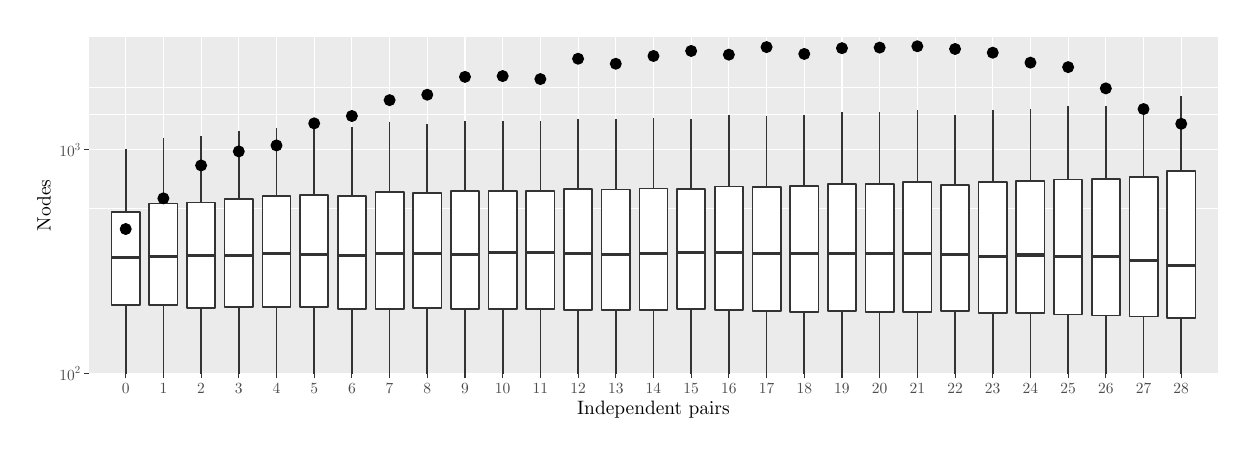
\begin{tikzpicture}[x=1pt,y=1pt]
\definecolor{fillColor}{RGB}{255,255,255}
\path[use as bounding box,fill=fillColor,fill opacity=0.00] (0,0) rectangle (433.62,144.54);
\begin{scope}
\path[clip] (  0.00,  0.00) rectangle (433.62,144.54);
\definecolor{drawColor}{RGB}{255,255,255}
\definecolor{fillColor}{RGB}{255,255,255}

\path[draw=drawColor,line width= 0.4pt,line join=round,line cap=round,fill=fillColor] ( -0.00,  0.00) rectangle (433.62,144.54);
\end{scope}
\begin{scope}
\path[clip] ( 22.14, 19.53) rectangle (430.12,141.04);
\definecolor{fillColor}{gray}{0.92}

\path[fill=fillColor] ( 22.14, 19.53) rectangle (430.12,141.04);
\definecolor{drawColor}{RGB}{255,255,255}

\path[draw=drawColor,line width= 0.2pt,line join=round] ( 22.14, 79.39) --
	(430.12, 79.39);

\path[draw=drawColor,line width= 0.2pt,line join=round] ( 22.14,113.42) --
	(430.12,113.42);

\path[draw=drawColor,line width= 0.2pt,line join=round] ( 22.14,122.92) --
	(430.12,122.92);

\path[draw=drawColor,line width= 0.4pt,line join=round] ( 22.14, 19.53) --
	(430.12, 19.53);

\path[draw=drawColor,line width= 0.4pt,line join=round] ( 22.14,100.38) --
	(430.12,100.38);

\path[draw=drawColor,line width= 0.4pt,line join=round] ( 35.42, 19.53) --
	( 35.42,141.04);

\path[draw=drawColor,line width= 0.4pt,line join=round] ( 49.04, 19.53) --
	( 49.04,141.04);

\path[draw=drawColor,line width= 0.4pt,line join=round] ( 62.67, 19.53) --
	( 62.67,141.04);

\path[draw=drawColor,line width= 0.4pt,line join=round] ( 76.29, 19.53) --
	( 76.29,141.04);

\path[draw=drawColor,line width= 0.4pt,line join=round] ( 89.91, 19.53) --
	( 89.91,141.04);

\path[draw=drawColor,line width= 0.4pt,line join=round] (103.53, 19.53) --
	(103.53,141.04);

\path[draw=drawColor,line width= 0.4pt,line join=round] (117.15, 19.53) --
	(117.15,141.04);

\path[draw=drawColor,line width= 0.4pt,line join=round] (130.78, 19.53) --
	(130.78,141.04);

\path[draw=drawColor,line width= 0.4pt,line join=round] (144.40, 19.53) --
	(144.40,141.04);

\path[draw=drawColor,line width= 0.4pt,line join=round] (158.02, 19.53) --
	(158.02,141.04);

\path[draw=drawColor,line width= 0.4pt,line join=round] (171.64, 19.53) --
	(171.64,141.04);

\path[draw=drawColor,line width= 0.4pt,line join=round] (185.26, 19.53) --
	(185.26,141.04);

\path[draw=drawColor,line width= 0.4pt,line join=round] (198.89, 19.53) --
	(198.89,141.04);

\path[draw=drawColor,line width= 0.4pt,line join=round] (212.51, 19.53) --
	(212.51,141.04);

\path[draw=drawColor,line width= 0.4pt,line join=round] (226.13, 19.53) --
	(226.13,141.04);

\path[draw=drawColor,line width= 0.4pt,line join=round] (239.75, 19.53) --
	(239.75,141.04);

\path[draw=drawColor,line width= 0.4pt,line join=round] (253.37, 19.53) --
	(253.37,141.04);

\path[draw=drawColor,line width= 0.4pt,line join=round] (267.00, 19.53) --
	(267.00,141.04);

\path[draw=drawColor,line width= 0.4pt,line join=round] (280.62, 19.53) --
	(280.62,141.04);

\path[draw=drawColor,line width= 0.4pt,line join=round] (294.24, 19.53) --
	(294.24,141.04);

\path[draw=drawColor,line width= 0.4pt,line join=round] (307.86, 19.53) --
	(307.86,141.04);

\path[draw=drawColor,line width= 0.4pt,line join=round] (321.48, 19.53) --
	(321.48,141.04);

\path[draw=drawColor,line width= 0.4pt,line join=round] (335.11, 19.53) --
	(335.11,141.04);

\path[draw=drawColor,line width= 0.4pt,line join=round] (348.73, 19.53) --
	(348.73,141.04);

\path[draw=drawColor,line width= 0.4pt,line join=round] (362.35, 19.53) --
	(362.35,141.04);

\path[draw=drawColor,line width= 0.4pt,line join=round] (375.97, 19.53) --
	(375.97,141.04);

\path[draw=drawColor,line width= 0.4pt,line join=round] (389.59, 19.53) --
	(389.59,141.04);

\path[draw=drawColor,line width= 0.4pt,line join=round] (403.22, 19.53) --
	(403.22,141.04);

\path[draw=drawColor,line width= 0.4pt,line join=round] (416.84, 19.53) --
	(416.84,141.04);
\definecolor{drawColor}{gray}{0.20}

\path[draw=drawColor,line width= 0.6pt,line join=round] ( 35.42, 77.89) --
	( 35.42,100.83);

\path[draw=drawColor,line width= 0.6pt,line join=round] ( 35.42, 44.22) --
	( 35.42, 32.09) --
	( 35.42, 13.41) --
	( 35.42,  0.00);
\definecolor{fillColor}{RGB}{255,255,255}

\path[draw=drawColor,line width= 0.6pt,line join=round,line cap=round,fill=fillColor] ( 30.31, 77.89) --
	( 30.31, 44.22) --
	( 35.42, 44.22) --
	( 40.53, 44.22) --
	( 40.53, 77.89) --
	( 35.42, 77.89) --
	( 30.31, 77.89) --
	cycle;

\path[draw=drawColor,line width= 1.1pt,line join=round] ( 30.31, 61.34) --
	( 35.42, 61.34) --
	( 40.53, 61.34);

\path[draw=drawColor,line width= 0.6pt,line join=round] ( 49.04, 80.95) --
	( 49.04,104.79);

\path[draw=drawColor,line width= 0.6pt,line join=round] ( 49.04, 44.22) --
	( 49.04, 25.49) --
	( 49.04,  0.00);

\path[draw=drawColor,line width= 0.6pt,line join=round,line cap=round,fill=fillColor] ( 43.94, 80.95) --
	( 43.94, 44.22) --
	( 49.04, 44.22) --
	( 54.15, 44.22) --
	( 54.15, 80.95) --
	( 49.04, 80.95) --
	( 43.94, 80.95) --
	cycle;

\path[draw=drawColor,line width= 1.1pt,line join=round] ( 43.94, 61.98) --
	( 49.04, 61.98) --
	( 54.15, 61.98);

\path[draw=drawColor,line width= 0.6pt,line join=round] ( 62.67, 81.37) --
	( 62.67,105.47);

\path[draw=drawColor,line width= 0.6pt,line join=round] ( 62.67, 43.33) --
	( 62.67, 23.51) --
	( 62.67,  0.00);

\path[draw=drawColor,line width= 0.6pt,line join=round,line cap=round,fill=fillColor] ( 57.56, 81.37) --
	( 57.56, 43.33) --
	( 62.67, 43.33) --
	( 67.77, 43.33) --
	( 67.77, 81.37) --
	( 62.67, 81.37) --
	( 57.56, 81.37) --
	cycle;

\path[draw=drawColor,line width= 1.1pt,line join=round] ( 57.56, 62.29) --
	( 62.67, 62.29) --
	( 67.77, 62.29);

\path[draw=drawColor,line width= 0.6pt,line join=round] ( 76.29, 82.62) --
	( 76.29,107.07);

\path[draw=drawColor,line width= 0.6pt,line join=round] ( 76.29, 43.51) --
	( 76.29, 24.13) --
	( 76.29,  0.00);

\path[draw=drawColor,line width= 0.6pt,line join=round,line cap=round,fill=fillColor] ( 71.18, 82.62) --
	( 71.18, 43.51) --
	( 76.29, 43.51) --
	( 81.40, 43.51) --
	( 81.40, 82.62) --
	( 76.29, 82.62) --
	( 71.18, 82.62) --
	cycle;

\path[draw=drawColor,line width= 1.1pt,line join=round] ( 71.18, 62.29) --
	( 76.29, 62.29) --
	( 81.40, 62.29);

\path[draw=drawColor,line width= 0.6pt,line join=round] ( 89.91, 83.65) --
	( 89.91,108.35);

\path[draw=drawColor,line width= 0.6pt,line join=round] ( 89.91, 43.51) --
	( 89.91, 24.13) --
	( 89.91,  0.00);

\path[draw=drawColor,line width= 0.6pt,line join=round,line cap=round,fill=fillColor] ( 84.80, 83.65) --
	( 84.80, 43.51) --
	( 89.91, 43.51) --
	( 95.02, 43.51) --
	( 95.02, 83.65) --
	( 89.91, 83.65) --
	( 84.80, 83.65) --
	cycle;

\path[draw=drawColor,line width= 1.1pt,line join=round] ( 84.80, 63.01) --
	( 89.91, 63.01) --
	( 95.02, 63.01);

\path[draw=drawColor,line width= 0.6pt,line join=round] (103.53, 84.04) --
	(103.53,108.80);

\path[draw=drawColor,line width= 0.6pt,line join=round] (103.53, 43.69) --
	(103.53, 23.97) --
	(103.53,  0.00);

\path[draw=drawColor,line width= 0.6pt,line join=round,line cap=round,fill=fillColor] ( 98.42, 84.04) --
	( 98.42, 43.69) --
	(103.53, 43.69) --
	(108.64, 43.69) --
	(108.64, 84.04) --
	(103.53, 84.04) --
	( 98.42, 84.04) --
	cycle;

\path[draw=drawColor,line width= 1.1pt,line join=round] ( 98.42, 62.70) --
	(103.53, 62.70) --
	(108.64, 62.70);

\path[draw=drawColor,line width= 0.6pt,line join=round] (117.15, 83.71) --
	(117.15,108.60);

\path[draw=drawColor,line width= 0.6pt,line join=round] (117.15, 42.80) --
	(117.15, 23.51) --
	(117.15,  0.00);

\path[draw=drawColor,line width= 0.6pt,line join=round,line cap=round,fill=fillColor] (112.05, 83.71) --
	(112.05, 42.80) --
	(117.15, 42.80) --
	(122.26, 42.80) --
	(122.26, 83.71) --
	(117.15, 83.71) --
	(112.05, 83.71) --
	cycle;

\path[draw=drawColor,line width= 1.1pt,line join=round] (112.05, 62.29) --
	(117.15, 62.29) --
	(122.26, 62.29);

\path[draw=drawColor,line width= 0.6pt,line join=round] (130.78, 85.20) --
	(130.78,110.42);

\path[draw=drawColor,line width= 0.6pt,line join=round] (130.78, 42.80) --
	(130.78, 23.82) --
	(130.78,  0.00);

\path[draw=drawColor,line width= 0.6pt,line join=round,line cap=round,fill=fillColor] (125.67, 85.20) --
	(125.67, 42.80) --
	(130.78, 42.80) --
	(135.88, 42.80) --
	(135.88, 85.20) --
	(130.78, 85.20) --
	(125.67, 85.20) --
	cycle;

\path[draw=drawColor,line width= 1.1pt,line join=round] (125.67, 62.81) --
	(130.78, 62.81) --
	(135.88, 62.81);

\path[draw=drawColor,line width= 0.6pt,line join=round] (144.40, 84.71) --
	(144.40,109.70);

\path[draw=drawColor,line width= 0.6pt,line join=round] (144.40, 43.33) --
	(144.40, 24.74) --
	(144.40,  0.00);

\path[draw=drawColor,line width= 0.6pt,line join=round,line cap=round,fill=fillColor] (139.29, 84.71) --
	(139.29, 43.33) --
	(144.40, 43.33) --
	(149.51, 43.33) --
	(149.51, 84.71) --
	(144.40, 84.71) --
	(139.29, 84.71) --
	cycle;

\path[draw=drawColor,line width= 1.1pt,line join=round] (139.29, 62.91) --
	(144.40, 62.91) --
	(149.51, 62.91);

\path[draw=drawColor,line width= 0.6pt,line join=round] (158.02, 85.52) --
	(158.02,110.81);

\path[draw=drawColor,line width= 0.6pt,line join=round] (158.02, 42.80) --
	(158.02, 23.35) --
	(158.02,  0.00);

\path[draw=drawColor,line width= 0.6pt,line join=round,line cap=round,fill=fillColor] (152.91, 85.52) --
	(152.91, 42.80) --
	(158.02, 42.80) --
	(163.13, 42.80) --
	(163.13, 85.52) --
	(158.02, 85.52) --
	(152.91, 85.52) --
	cycle;

\path[draw=drawColor,line width= 1.1pt,line join=round] (152.91, 62.70) --
	(158.02, 62.70) --
	(163.13, 62.70);

\path[draw=drawColor,line width= 0.6pt,line join=round] (171.64, 85.52) --
	(171.64,110.65);

\path[draw=drawColor,line width= 0.6pt,line join=round] (171.64, 42.98) --
	(171.64, 30.84) --
	(171.64, 12.13) --
	(171.64,  0.00);

\path[draw=drawColor,line width= 0.6pt,line join=round,line cap=round,fill=fillColor] (166.53, 85.52) --
	(166.53, 42.98) --
	(171.64, 42.98) --
	(176.75, 42.98) --
	(176.75, 85.52) --
	(171.64, 85.52) --
	(166.53, 85.52) --
	cycle;

\path[draw=drawColor,line width= 1.1pt,line join=round] (166.53, 63.21) --
	(171.64, 63.21) --
	(176.75, 63.21);

\path[draw=drawColor,line width= 0.6pt,line join=round] (185.26, 85.63) --
	(185.26,110.94);

\path[draw=drawColor,line width= 0.6pt,line join=round] (185.26, 42.80) --
	(185.26, 23.82) --
	(185.26,  0.00);

\path[draw=drawColor,line width= 0.6pt,line join=round,line cap=round,fill=fillColor] (180.16, 85.63) --
	(180.16, 42.80) --
	(185.26, 42.80) --
	(190.37, 42.80) --
	(190.37, 85.63) --
	(185.26, 85.63) --
	(180.16, 85.63) --
	cycle;

\path[draw=drawColor,line width= 1.1pt,line join=round] (180.16, 63.21) --
	(185.26, 63.21) --
	(190.37, 63.21);

\path[draw=drawColor,line width= 0.6pt,line join=round] (198.89, 86.17) --
	(198.89,111.64);

\path[draw=drawColor,line width= 0.6pt,line join=round] (198.89, 42.61) --
	(198.89, 23.19) --
	(198.89,  0.00);

\path[draw=drawColor,line width= 0.6pt,line join=round,line cap=round,fill=fillColor] (193.78, 86.17) --
	(193.78, 42.61) --
	(198.89, 42.61) --
	(203.99, 42.61) --
	(203.99, 86.17) --
	(198.89, 86.17) --
	(193.78, 86.17) --
	cycle;

\path[draw=drawColor,line width= 1.1pt,line join=round] (193.78, 62.91) --
	(198.89, 62.91) --
	(203.99, 62.91);

\path[draw=drawColor,line width= 0.6pt,line join=round] (212.51, 86.11) --
	(212.51,111.59);

\path[draw=drawColor,line width= 0.6pt,line join=round] (212.51, 42.43) --
	(212.51, 23.35) --
	(212.51,  0.00);

\path[draw=drawColor,line width= 0.6pt,line join=round,line cap=round,fill=fillColor] (207.40, 86.11) --
	(207.40, 42.43) --
	(212.51, 42.43) --
	(217.62, 42.43) --
	(217.62, 86.11) --
	(212.51, 86.11) --
	(207.40, 86.11) --
	cycle;

\path[draw=drawColor,line width= 1.1pt,line join=round] (207.40, 62.50) --
	(212.51, 62.50) --
	(217.62, 62.50);

\path[draw=drawColor,line width= 0.6pt,line join=round] (226.13, 86.42) --
	(226.13,111.81);

\path[draw=drawColor,line width= 0.6pt,line join=round] (226.13, 42.61) --
	(226.13, 23.82) --
	(226.13,  0.00);

\path[draw=drawColor,line width= 0.6pt,line join=round,line cap=round,fill=fillColor] (221.02, 86.42) --
	(221.02, 42.61) --
	(226.13, 42.61) --
	(231.24, 42.61) --
	(231.24, 86.42) --
	(226.13, 86.42) --
	(221.02, 86.42) --
	cycle;

\path[draw=drawColor,line width= 1.1pt,line join=round] (221.02, 62.91) --
	(226.13, 62.91) --
	(231.24, 62.91);

\path[draw=drawColor,line width= 0.6pt,line join=round] (239.75, 86.32) --
	(239.75,111.71);

\path[draw=drawColor,line width= 0.6pt,line join=round] (239.75, 42.98) --
	(239.75, 24.13) --
	(239.75,  0.00);

\path[draw=drawColor,line width= 0.6pt,line join=round,line cap=round,fill=fillColor] (234.64, 86.32) --
	(234.64, 42.98) --
	(239.75, 42.98) --
	(244.86, 42.98) --
	(244.86, 86.32) --
	(239.75, 86.32) --
	(234.64, 86.32) --
	cycle;

\path[draw=drawColor,line width= 1.1pt,line join=round] (234.64, 63.21) --
	(239.75, 63.21) --
	(244.86, 63.21);

\path[draw=drawColor,line width= 0.6pt,line join=round] (253.37, 87.11) --
	(253.37,112.81);

\path[draw=drawColor,line width= 0.6pt,line join=round] (253.37, 42.43) --
	(253.37, 23.19) --
	(253.37,  0.00);

\path[draw=drawColor,line width= 0.6pt,line join=round,line cap=round,fill=fillColor] (248.27, 87.11) --
	(248.27, 42.43) --
	(253.37, 42.43) --
	(258.48, 42.43) --
	(258.48, 87.11) --
	(253.37, 87.11) --
	(248.27, 87.11) --
	cycle;

\path[draw=drawColor,line width= 1.1pt,line join=round] (248.27, 63.26) --
	(253.37, 63.26) --
	(258.48, 63.26);

\path[draw=drawColor,line width= 0.6pt,line join=round] (267.00, 87.00) --
	(267.00,112.67);

\path[draw=drawColor,line width= 0.6pt,line join=round] (267.00, 42.25) --
	(267.00, 23.82) --
	(267.00,  0.00);

\path[draw=drawColor,line width= 0.6pt,line join=round,line cap=round,fill=fillColor] (261.89, 87.00) --
	(261.89, 42.25) --
	(267.00, 42.25) --
	(272.10, 42.25) --
	(272.10, 87.00) --
	(267.00, 87.00) --
	(261.89, 87.00) --
	cycle;

\path[draw=drawColor,line width= 1.1pt,line join=round] (261.89, 62.91) --
	(267.00, 62.91) --
	(272.10, 62.91);

\path[draw=drawColor,line width= 0.6pt,line join=round] (280.62, 87.31) --
	(280.62,113.16);

\path[draw=drawColor,line width= 0.6pt,line join=round] (280.62, 41.88) --
	(280.62, 22.87) --
	(280.62,  0.00);

\path[draw=drawColor,line width= 0.6pt,line join=round,line cap=round,fill=fillColor] (275.51, 87.31) --
	(275.51, 41.88) --
	(280.62, 41.88) --
	(285.73, 41.88) --
	(285.73, 87.31) --
	(280.62, 87.31) --
	(275.51, 87.31) --
	cycle;

\path[draw=drawColor,line width= 1.1pt,line join=round] (275.51, 62.81) --
	(280.62, 62.81) --
	(285.73, 62.81);

\path[draw=drawColor,line width= 0.6pt,line join=round] (294.24, 88.10) --
	(294.24,113.98);

\path[draw=drawColor,line width= 0.6pt,line join=round] (294.24, 42.25) --
	(294.24, 23.19) --
	(294.24,  0.00);

\path[draw=drawColor,line width= 0.6pt,line join=round,line cap=round,fill=fillColor] (289.13, 88.10) --
	(289.13, 42.25) --
	(294.24, 42.25) --
	(299.35, 42.25) --
	(299.35, 88.10) --
	(294.24, 88.10) --
	(289.13, 88.10) --
	cycle;

\path[draw=drawColor,line width= 1.1pt,line join=round] (289.13, 63.01) --
	(294.24, 63.01) --
	(299.35, 63.01);

\path[draw=drawColor,line width= 0.6pt,line join=round] (307.86, 87.97) --
	(307.86,113.91);

\path[draw=drawColor,line width= 0.6pt,line join=round] (307.86, 41.88) --
	(307.86, 22.39) --
	(307.86,  0.00);

\path[draw=drawColor,line width= 0.6pt,line join=round,line cap=round,fill=fillColor] (302.75, 87.97) --
	(302.75, 41.88) --
	(307.86, 41.88) --
	(312.97, 41.88) --
	(312.97, 87.97) --
	(307.86, 87.97) --
	(302.75, 87.97) --
	cycle;

\path[draw=drawColor,line width= 1.1pt,line join=round] (302.75, 62.81) --
	(307.86, 62.81) --
	(312.97, 62.81);

\path[draw=drawColor,line width= 0.6pt,line join=round] (321.48, 88.70) --
	(321.48,114.80);

\path[draw=drawColor,line width= 0.6pt,line join=round] (321.48, 41.69) --
	(321.48, 22.39) --
	(321.48,  0.00);

\path[draw=drawColor,line width= 0.6pt,line join=round,line cap=round,fill=fillColor] (316.38, 88.70) --
	(316.38, 41.69) --
	(321.48, 41.69) --
	(326.59, 41.69) --
	(326.59, 88.70) --
	(321.48, 88.70) --
	(316.38, 88.70) --
	cycle;

\path[draw=drawColor,line width= 1.1pt,line join=round] (316.38, 62.81) --
	(321.48, 62.81) --
	(326.59, 62.81);

\path[draw=drawColor,line width= 0.6pt,line join=round] (335.11, 87.70) --
	(335.11,113.08);

\path[draw=drawColor,line width= 0.6pt,line join=round] (335.11, 42.06) --
	(335.11, 23.19) --
	(335.11,  0.00);

\path[draw=drawColor,line width= 0.6pt,line join=round,line cap=round,fill=fillColor] (330.00, 87.70) --
	(330.00, 42.06) --
	(335.11, 42.06) --
	(340.21, 42.06) --
	(340.21, 87.70) --
	(335.11, 87.70) --
	(330.00, 87.70) --
	cycle;

\path[draw=drawColor,line width= 1.1pt,line join=round] (330.00, 62.60) --
	(335.11, 62.60) --
	(340.21, 62.60);

\path[draw=drawColor,line width= 0.6pt,line join=round] (348.73, 88.75) --
	(348.73,114.92);

\path[draw=drawColor,line width= 0.6pt,line join=round] (348.73, 41.51) --
	(348.73, 22.55) --
	(348.73,  0.00);

\path[draw=drawColor,line width= 0.6pt,line join=round,line cap=round,fill=fillColor] (343.62, 88.75) --
	(343.62, 41.51) --
	(348.73, 41.51) --
	(353.84, 41.51) --
	(353.84, 88.75) --
	(348.73, 88.75) --
	(343.62, 88.75) --
	cycle;

\path[draw=drawColor,line width= 1.1pt,line join=round] (343.62, 61.98) --
	(348.73, 61.98) --
	(353.84, 61.98);

\path[draw=drawColor,line width= 0.6pt,line join=round] (362.35, 89.04) --
	(362.35,115.15);

\path[draw=drawColor,line width= 0.6pt,line join=round] (362.35, 41.32) --
	(362.35, 22.39) --
	(362.35,  0.00);

\path[draw=drawColor,line width= 0.6pt,line join=round,line cap=round,fill=fillColor] (357.24, 89.04) --
	(357.24, 41.32) --
	(362.35, 41.32) --
	(367.46, 41.32) --
	(367.46, 89.04) --
	(362.35, 89.04) --
	(357.24, 89.04) --
	cycle;

\path[draw=drawColor,line width= 1.1pt,line join=round] (357.24, 62.39) --
	(362.35, 62.39) --
	(367.46, 62.39);

\path[draw=drawColor,line width= 0.6pt,line join=round] (375.97, 89.66) --
	(375.97,116.10);

\path[draw=drawColor,line width= 0.6pt,line join=round] (375.97, 40.94) --
	(375.97, 22.87) --
	(375.97,  0.00);

\path[draw=drawColor,line width= 0.6pt,line join=round,line cap=round,fill=fillColor] (370.86, 89.66) --
	(370.86, 73.15) --
	(370.86, 40.94) --
	(375.97, 40.94) --
	(381.08, 40.94) --
	(381.08, 73.15) --
	(381.08, 89.66) --
	(375.97, 89.66) --
	(370.86, 89.66) --
	cycle;

\path[draw=drawColor,line width= 1.1pt,line join=round] (370.86, 61.98) --
	(375.97, 61.98) --
	(381.08, 61.98);

\path[draw=drawColor,line width= 0.6pt,line join=round] (389.59, 89.81) --
	(389.59,116.33);

\path[draw=drawColor,line width= 0.6pt,line join=round] (389.59, 40.55) --
	(389.59, 21.41) --
	(389.59,  0.00);

\path[draw=drawColor,line width= 0.6pt,line join=round,line cap=round,fill=fillColor] (384.49, 89.81) --
	(384.49, 73.19) --
	(384.49, 40.55) --
	(389.59, 40.55) --
	(394.70, 40.55) --
	(394.70, 73.19) --
	(394.70, 89.81) --
	(389.59, 89.81) --
	(384.49, 89.81) --
	cycle;

\path[draw=drawColor,line width= 1.1pt,line join=round] (384.49, 61.77) --
	(389.59, 61.77) --
	(394.70, 61.77);

\path[draw=drawColor,line width= 0.6pt,line join=round] (403.22, 90.61) --
	(403.22,117.36);

\path[draw=drawColor,line width= 0.6pt,line join=round] (403.22, 40.17) --
	(403.22, 21.57) --
	(403.22,  0.00);

\path[draw=drawColor,line width= 0.6pt,line join=round,line cap=round,fill=fillColor] (398.11, 90.61) --
	(398.11, 73.76) --
	(398.11, 40.17) --
	(403.22, 40.17) --
	(408.32, 40.17) --
	(408.32, 73.76) --
	(408.32, 90.61) --
	(403.22, 90.61) --
	(398.11, 90.61) --
	cycle;

\path[draw=drawColor,line width= 1.1pt,line join=round] (398.11, 60.26) --
	(403.22, 60.26) --
	(408.32, 60.26);

\path[draw=drawColor,line width= 0.6pt,line join=round] (416.84, 92.67) --
	(416.84,119.87);

\path[draw=drawColor,line width= 0.6pt,line join=round] (416.84, 39.58) --
	(416.84, 20.74) --
	(416.84,  0.00);

\path[draw=drawColor,line width= 0.6pt,line join=round,line cap=round,fill=fillColor] (411.73, 92.67) --
	(411.73, 75.33) --
	(411.73, 39.58) --
	(416.84, 39.58) --
	(421.95, 39.58) --
	(421.95, 75.33) --
	(421.95, 92.67) --
	(416.84, 92.67) --
	(411.73, 92.67) --
	cycle;

\path[draw=drawColor,line width= 1.1pt,line join=round] (411.73, 58.57) --
	(416.84, 58.57) --
	(421.95, 58.57);
\definecolor{drawColor}{RGB}{0,0,0}
\definecolor{fillColor}{RGB}{0,0,0}

\path[draw=drawColor,line width= 0.4pt,line join=round,line cap=round,fill=fillColor] ( 35.42, 71.78) circle (  1.96);

\path[draw=drawColor,line width= 0.4pt,line join=round,line cap=round,fill=fillColor] ( 49.04, 82.87) circle (  1.96);

\path[draw=drawColor,line width= 0.4pt,line join=round,line cap=round,fill=fillColor] ( 62.67, 94.76) circle (  1.96);

\path[draw=drawColor,line width= 0.4pt,line join=round,line cap=round,fill=fillColor] ( 76.29, 99.83) circle (  1.96);

\path[draw=drawColor,line width= 0.4pt,line join=round,line cap=round,fill=fillColor] ( 89.91,101.99) circle (  1.96);

\path[draw=drawColor,line width= 0.4pt,line join=round,line cap=round,fill=fillColor] (103.53,109.96) circle (  1.96);

\path[draw=drawColor,line width= 0.4pt,line join=round,line cap=round,fill=fillColor] (117.15,112.62) circle (  1.96);

\path[draw=drawColor,line width= 0.4pt,line join=round,line cap=round,fill=fillColor] (130.78,118.35) circle (  1.96);

\path[draw=drawColor,line width= 0.4pt,line join=round,line cap=round,fill=fillColor] (144.40,120.31) circle (  1.96);

\path[draw=drawColor,line width= 0.4pt,line join=round,line cap=round,fill=fillColor] (158.02,126.76) circle (  1.96);

\path[draw=drawColor,line width= 0.4pt,line join=round,line cap=round,fill=fillColor] (171.64,127.05) circle (  1.96);

\path[draw=drawColor,line width= 0.4pt,line join=round,line cap=round,fill=fillColor] (185.26,125.96) circle (  1.96);

\path[draw=drawColor,line width= 0.4pt,line join=round,line cap=round,fill=fillColor] (198.89,133.31) circle (  1.96);

\path[draw=drawColor,line width= 0.4pt,line join=round,line cap=round,fill=fillColor] (212.51,131.50) circle (  1.96);

\path[draw=drawColor,line width= 0.4pt,line join=round,line cap=round,fill=fillColor] (226.13,134.31) circle (  1.96);

\path[draw=drawColor,line width= 0.4pt,line join=round,line cap=round,fill=fillColor] (239.75,136.12) circle (  1.96);

\path[draw=drawColor,line width= 0.4pt,line join=round,line cap=round,fill=fillColor] (253.37,134.78) circle (  1.96);

\path[draw=drawColor,line width= 0.4pt,line join=round,line cap=round,fill=fillColor] (267.00,137.52) circle (  1.96);

\path[draw=drawColor,line width= 0.4pt,line join=round,line cap=round,fill=fillColor] (280.62,135.05) circle (  1.96);

\path[draw=drawColor,line width= 0.4pt,line join=round,line cap=round,fill=fillColor] (294.24,137.13) circle (  1.96);

\path[draw=drawColor,line width= 0.4pt,line join=round,line cap=round,fill=fillColor] (307.86,137.34) circle (  1.96);

\path[draw=drawColor,line width= 0.4pt,line join=round,line cap=round,fill=fillColor] (321.48,137.82) circle (  1.96);

\path[draw=drawColor,line width= 0.4pt,line join=round,line cap=round,fill=fillColor] (335.11,136.84) circle (  1.96);

\path[draw=drawColor,line width= 0.4pt,line join=round,line cap=round,fill=fillColor] (348.73,135.50) circle (  1.96);

\path[draw=drawColor,line width= 0.4pt,line join=round,line cap=round,fill=fillColor] (362.35,131.90) circle (  1.96);

\path[draw=drawColor,line width= 0.4pt,line join=round,line cap=round,fill=fillColor] (375.97,130.28) circle (  1.96);

\path[draw=drawColor,line width= 0.4pt,line join=round,line cap=round,fill=fillColor] (389.59,122.60) circle (  1.96);

\path[draw=drawColor,line width= 0.4pt,line join=round,line cap=round,fill=fillColor] (403.22,115.13) circle (  1.96);

\path[draw=drawColor,line width= 0.4pt,line join=round,line cap=round,fill=fillColor] (416.84,109.80) circle (  1.96);
\end{scope}
\begin{scope}
\path[clip] (  0.00,  0.00) rectangle (433.62,144.54);
\definecolor{drawColor}{gray}{0.30}

\node[text=drawColor,anchor=base west,inner sep=0pt, outer sep=0pt, scale=  0.56] at ( 11.43, 17.12) {10};

\node[text=drawColor,anchor=base west,inner sep=0pt, outer sep=0pt, scale=  0.39] at ( 17.03, 19.41) {2};

\node[text=drawColor,anchor=base west,inner sep=0pt, outer sep=0pt, scale=  0.56] at ( 11.43, 97.98) {10};

\node[text=drawColor,anchor=base west,inner sep=0pt, outer sep=0pt, scale=  0.39] at ( 17.03,100.27) {3};
\end{scope}
\begin{scope}
\path[clip] (  0.00,  0.00) rectangle (433.62,144.54);
\definecolor{drawColor}{gray}{0.20}

\path[draw=drawColor,line width= 0.4pt,line join=round] ( 20.39, 19.53) --
	( 22.14, 19.53);

\path[draw=drawColor,line width= 0.4pt,line join=round] ( 20.39,100.38) --
	( 22.14,100.38);
\end{scope}
\begin{scope}
\path[clip] (  0.00,  0.00) rectangle (433.62,144.54);
\definecolor{drawColor}{gray}{0.20}

\path[draw=drawColor,line width= 0.4pt,line join=round] ( 35.42, 17.78) --
	( 35.42, 19.53);

\path[draw=drawColor,line width= 0.4pt,line join=round] ( 49.04, 17.78) --
	( 49.04, 19.53);

\path[draw=drawColor,line width= 0.4pt,line join=round] ( 62.67, 17.78) --
	( 62.67, 19.53);

\path[draw=drawColor,line width= 0.4pt,line join=round] ( 76.29, 17.78) --
	( 76.29, 19.53);

\path[draw=drawColor,line width= 0.4pt,line join=round] ( 89.91, 17.78) --
	( 89.91, 19.53);

\path[draw=drawColor,line width= 0.4pt,line join=round] (103.53, 17.78) --
	(103.53, 19.53);

\path[draw=drawColor,line width= 0.4pt,line join=round] (117.15, 17.78) --
	(117.15, 19.53);

\path[draw=drawColor,line width= 0.4pt,line join=round] (130.78, 17.78) --
	(130.78, 19.53);

\path[draw=drawColor,line width= 0.4pt,line join=round] (144.40, 17.78) --
	(144.40, 19.53);

\path[draw=drawColor,line width= 0.4pt,line join=round] (158.02, 17.78) --
	(158.02, 19.53);

\path[draw=drawColor,line width= 0.4pt,line join=round] (171.64, 17.78) --
	(171.64, 19.53);

\path[draw=drawColor,line width= 0.4pt,line join=round] (185.26, 17.78) --
	(185.26, 19.53);

\path[draw=drawColor,line width= 0.4pt,line join=round] (198.89, 17.78) --
	(198.89, 19.53);

\path[draw=drawColor,line width= 0.4pt,line join=round] (212.51, 17.78) --
	(212.51, 19.53);

\path[draw=drawColor,line width= 0.4pt,line join=round] (226.13, 17.78) --
	(226.13, 19.53);

\path[draw=drawColor,line width= 0.4pt,line join=round] (239.75, 17.78) --
	(239.75, 19.53);

\path[draw=drawColor,line width= 0.4pt,line join=round] (253.37, 17.78) --
	(253.37, 19.53);

\path[draw=drawColor,line width= 0.4pt,line join=round] (267.00, 17.78) --
	(267.00, 19.53);

\path[draw=drawColor,line width= 0.4pt,line join=round] (280.62, 17.78) --
	(280.62, 19.53);

\path[draw=drawColor,line width= 0.4pt,line join=round] (294.24, 17.78) --
	(294.24, 19.53);

\path[draw=drawColor,line width= 0.4pt,line join=round] (307.86, 17.78) --
	(307.86, 19.53);

\path[draw=drawColor,line width= 0.4pt,line join=round] (321.48, 17.78) --
	(321.48, 19.53);

\path[draw=drawColor,line width= 0.4pt,line join=round] (335.11, 17.78) --
	(335.11, 19.53);

\path[draw=drawColor,line width= 0.4pt,line join=round] (348.73, 17.78) --
	(348.73, 19.53);

\path[draw=drawColor,line width= 0.4pt,line join=round] (362.35, 17.78) --
	(362.35, 19.53);

\path[draw=drawColor,line width= 0.4pt,line join=round] (375.97, 17.78) --
	(375.97, 19.53);

\path[draw=drawColor,line width= 0.4pt,line join=round] (389.59, 17.78) --
	(389.59, 19.53);

\path[draw=drawColor,line width= 0.4pt,line join=round] (403.22, 17.78) --
	(403.22, 19.53);

\path[draw=drawColor,line width= 0.4pt,line join=round] (416.84, 17.78) --
	(416.84, 19.53);
\end{scope}
\begin{scope}
\path[clip] (  0.00,  0.00) rectangle (433.62,144.54);
\definecolor{drawColor}{gray}{0.30}

\node[text=drawColor,anchor=base,inner sep=0pt, outer sep=0pt, scale=  0.56] at ( 35.42, 12.52) {0};

\node[text=drawColor,anchor=base,inner sep=0pt, outer sep=0pt, scale=  0.56] at ( 49.04, 12.52) {1};

\node[text=drawColor,anchor=base,inner sep=0pt, outer sep=0pt, scale=  0.56] at ( 62.67, 12.52) {2};

\node[text=drawColor,anchor=base,inner sep=0pt, outer sep=0pt, scale=  0.56] at ( 76.29, 12.52) {3};

\node[text=drawColor,anchor=base,inner sep=0pt, outer sep=0pt, scale=  0.56] at ( 89.91, 12.52) {4};

\node[text=drawColor,anchor=base,inner sep=0pt, outer sep=0pt, scale=  0.56] at (103.53, 12.52) {5};

\node[text=drawColor,anchor=base,inner sep=0pt, outer sep=0pt, scale=  0.56] at (117.15, 12.52) {6};

\node[text=drawColor,anchor=base,inner sep=0pt, outer sep=0pt, scale=  0.56] at (130.78, 12.52) {7};

\node[text=drawColor,anchor=base,inner sep=0pt, outer sep=0pt, scale=  0.56] at (144.40, 12.52) {8};

\node[text=drawColor,anchor=base,inner sep=0pt, outer sep=0pt, scale=  0.56] at (158.02, 12.52) {9};

\node[text=drawColor,anchor=base,inner sep=0pt, outer sep=0pt, scale=  0.56] at (171.64, 12.52) {10};

\node[text=drawColor,anchor=base,inner sep=0pt, outer sep=0pt, scale=  0.56] at (185.26, 12.52) {11};

\node[text=drawColor,anchor=base,inner sep=0pt, outer sep=0pt, scale=  0.56] at (198.89, 12.52) {12};

\node[text=drawColor,anchor=base,inner sep=0pt, outer sep=0pt, scale=  0.56] at (212.51, 12.52) {13};

\node[text=drawColor,anchor=base,inner sep=0pt, outer sep=0pt, scale=  0.56] at (226.13, 12.52) {14};

\node[text=drawColor,anchor=base,inner sep=0pt, outer sep=0pt, scale=  0.56] at (239.75, 12.52) {15};

\node[text=drawColor,anchor=base,inner sep=0pt, outer sep=0pt, scale=  0.56] at (253.37, 12.52) {16};

\node[text=drawColor,anchor=base,inner sep=0pt, outer sep=0pt, scale=  0.56] at (267.00, 12.52) {17};

\node[text=drawColor,anchor=base,inner sep=0pt, outer sep=0pt, scale=  0.56] at (280.62, 12.52) {18};

\node[text=drawColor,anchor=base,inner sep=0pt, outer sep=0pt, scale=  0.56] at (294.24, 12.52) {19};

\node[text=drawColor,anchor=base,inner sep=0pt, outer sep=0pt, scale=  0.56] at (307.86, 12.52) {20};

\node[text=drawColor,anchor=base,inner sep=0pt, outer sep=0pt, scale=  0.56] at (321.48, 12.52) {21};

\node[text=drawColor,anchor=base,inner sep=0pt, outer sep=0pt, scale=  0.56] at (335.11, 12.52) {22};

\node[text=drawColor,anchor=base,inner sep=0pt, outer sep=0pt, scale=  0.56] at (348.73, 12.52) {23};

\node[text=drawColor,anchor=base,inner sep=0pt, outer sep=0pt, scale=  0.56] at (362.35, 12.52) {24};

\node[text=drawColor,anchor=base,inner sep=0pt, outer sep=0pt, scale=  0.56] at (375.97, 12.52) {25};

\node[text=drawColor,anchor=base,inner sep=0pt, outer sep=0pt, scale=  0.56] at (389.59, 12.52) {26};

\node[text=drawColor,anchor=base,inner sep=0pt, outer sep=0pt, scale=  0.56] at (403.22, 12.52) {27};

\node[text=drawColor,anchor=base,inner sep=0pt, outer sep=0pt, scale=  0.56] at (416.84, 12.52) {28};
\end{scope}
\begin{scope}
\path[clip] (  0.00,  0.00) rectangle (433.62,144.54);
\definecolor{drawColor}{RGB}{0,0,0}

\node[text=drawColor,anchor=base,inner sep=0pt, outer sep=0pt, scale=  0.70] at (226.13,  4.86) {Independent pairs};
\end{scope}
\begin{scope}
\path[clip] (  0.00,  0.00) rectangle (433.62,144.54);
\definecolor{drawColor}{RGB}{0,0,0}

\node[text=drawColor,rotate= 90.00,anchor=base,inner sep=0pt, outer sep=0pt, scale=  0.70] at (  8.32, 80.28) {Nodes};
\end{scope}
\end{tikzpicture}

  \caption{The distribution of the number of nodes in the binary search tree as
    a function of the number of independent pairs of predicates for
    $|\predicates| = 8$. Outliers are hidden, the dots denote mean values, and
    the vertical axis is on a $\log_{10}$ scale.}
  \label{fig:phase_transition}
\end{figure*}

Along with constraints, variables, and their domains, two more design decisions
are needed to complete the model: heuristics and restarts. By trial and error,
the variable ordering heuristic was devised to eliminate sources of thrashing,
i.e., situations where a contradiction is being `fixed' by making changes that
have no hope to fix the contradiction. Thus, we partition all decision variables
into an ordered list of groups, and require the values of all variables from one
group to be determined before moving to the next group. Within each group, we
use the `fail first' variable ordering heuristic. The first group consists of
all head predicates. Afterwards, we handle all remaining decision variables from
the first clause before proceeding to the next. The decision variables within
each clause are divided into:
\begin{enumerate*}
\item the $\variable{structure}$ array,
\item body predicates,
\item head arguments,
\item (if $|\variables{}| > 1$) the $\variable{intros}$ array,
\item body arguments.
\end{enumerate*}
For instance, in the clause from \cref{example:sibling}, all visible parts of
the clause would be decided in this order:
\[
  \overset{1}{\mathsf{sibling}}(\overset{3}{X}, \overset{3}{Y}) \gets
  \overset{2}{\mathsf{parent}}(\overset{4}{X}, \overset{4}{Z})
  \overset{2}{\land} \overset{2}{\mathsf{parent}}(\overset{4}{Y},
  \overset{4}{Z}).
\]
We also employ a geometric restart policy, restarting after $10, 20, 40,
80, \dots$ contradictions.

We ran close to \num{400000} experiments, investigating whether the model is
efficient enough to generate reasonably-sized programs and gaining insight into
what parameter values make the constraint satisfaction problem harder. For these
experiments, we use Choco~4.10.2 \citep{choco} with Java~8 on a computer with an
Intel Core i5-8250U processor. For $|\predicates{}|$, $|\variables{}|$,
$|\constants{}|$, $\maxNumNodes{}$, and $\maxNumClauses{} - |\predicates{}|$
(i.e., the number of clauses in addition to the mandatory $|\predicates{}|$
clauses), we assign all combinations of 1, 2, 4, 8. $\maxArity{}$ is assigned to
values 1--4. For each $|\predicates{}|$, we also iterate over all possible
numbers of independent pairs of predicates, ranging from 0 up to
$\binom{|\predicates{}|}{2}$. For each combination of the above-mentioned
parameters, we pick ten random ways to assign arities to predicates (such that
$\maxArity{}$ occurs at least once) and ten random combinations of independent
pairs. We then run the solver with a \SI{60}{\second} timeout.

The vast majority (\SI{97.7}{\percent}) of runs finished in under
\SI{1}{\second}, while four instances timed out: all with $|\predicates| =
\maxNumClauses{} - |\predicates{}| = \maxNumNodes{} = 8$ and the remaining
parameters all different. This suggests that---regardless of parameter
values---most of the time a solution can be identified instantaneously while
occasionally a series of wrong decisions can lead the solver into a part of the
search space with no solutions.

In \cref{fig:impact}, we plot how the mean number of nodes in the binary search
tree grows as a function of each parameter (the plot for the median is very
similar). The growth of each curve suggest how well/poorly the model scales with
higher values of the parameter. From this plot, it is clear that
$\maxNumNodes{}$ is the limiting factor. This is because some tree structures
can be impossible to fill with predicates without creating either a negative
cycle or a forbidden dependency, and such trees become more common as the number
of nodes increases. Likewise, a higher number of predicates complicates the
situation as well.

\cref{fig:phase_transition} takes the data for $|\predicates{}| = 8$ (almost
\num{300000} observations) and shows how the number of nodes in the search tree
varies with the number of independent pairs of predicates. The box plots show
that the median number of nodes stays about the same while the dots
(representing the means) draw an arc. This suggests a type of phase transition,
but only in mean rather than median, i.e., most problems remain easy, but with
some parameter values hard problems become more likely. On the one hand, with
few pairs of independent predicates, one can easily find the right combination
of predicates to use in each clause. On the other hand, if most predicates must
be independent, this leaves fewer predicates that can be used in the body of
each clause (since all of them have to be independent with the head predicate),
and we can either quickly find a solution or identify that there is none.

% TODO: talk about randomness. The value heuristic is random because we want
% randomness. After finding one solution, one can continue the search for more,
% but they will be similar (acceptable if the search space is small and we want
% to find all solutions).
% On the other hand, with restarts, duplicates become possible.

\section{CONCLUSIONS}
% TODO (Fazl): equations and 'provides no such guarantees' sound more like
% future work / limitation section. Make it sound more positive.

We were able to design an efficient model for generating both logic programs and
probabilistic logic programs. The model avoids unnecessary symmetries, generates
valid programs, and can ensure predicate independence. Note that there is one
kind of symmetries not handled by our model, i.e., logical equivalence. For
example, all three of these formulas are logically equivalent but syntactically
different: $\neg(\mathsf{P}(X) \lor \mathsf{Q}(X))$, $\neg\mathsf{P}(X) \land
\neg\mathsf{Q}(X)$, and $\neg\mathsf{Q}(X) \land \neg\mathsf{P}(X)$. While there
are many situations where one would prefer to treat logically equivalent
formulas as symmetries that should be eliminated, there are also situations
where we do care about enumerating different ways to express the same
probability distribution or knowledge base. For instance, one could look for the
`best' logically equivalent formula, or investigate whether some formulas result
in faster inference than others.

Another issue worth discussing is that of randomness. Most random models sample
from a well-defined probability distribution whereas a constraint model, while
potentially sufficiently random, provides no such guarantees. In future work, it
would be interesting to examine the probability distribution of logic programs
as generated by our model, although it is not obvious how such a
probability distribution could be characterised.% One example of a clear bias
%exhibited by our model is that of complexity over simplicity, i.e., if a tree
%that represents the body of a clause can have up to $\maxNumNodes{}$
%nodes---because the number of possible trees with $n$ nodes grows with $n$---it
%is much more likely to have $\maxNumNodes{}$ or $\maxNumNodes{} - 1$ nodes than,
%e.g., one or two.

% TODO: We can do the same thing for predicates within the body of a clause that
% we do with variables, i.e., predicates within a clause are permutable (except
% for the head predicate), so we can have a set of 'allowed' predicates.

%\subsubsection*{Acknowledgements}

%This work was supported by the EPSRC Centre for Doctoral Training in
%Robotics and Autonomous Systems, funded by the UK Engineering and Physical
%Sciences Research Council (grant EP/S023208/1).

\renewcommand{\bibsection}{\subsubsection*{References}}
\bibliography{paper}
% TODO: logic programs don't have disjunctions. Is there an easy way to
% eliminate them?

\appendix
\section{EXAMPLE PROGRAMS}

In this appendix, we provide examples of probabilistic logic programs generated
by various combinations of parameters. In all cases, we use $\{ 0.1, 0.2, \dots,
0.9, 1, 1, 1, 1, 1\}$ as the multiset of probabilities. Each clause is written
on a separate line and ends with a full stop. The head and the body of each
clause are separated with \texttt{:-} (instead of $\gets$). The probability of
each clause is prepended to the clause, using \texttt{::} as a separator.
Probabilities equal to one and empty bodies of clauses can be omitted.
Conjunction, disjunction, and negation are denoted by commas, semicolons, and
`\texttt{\textbackslash+}', respectively. Parentheses are used to demonstrate
precedence, although many of them are redundant. 

By setting $\predicates{} = [\texttt{p}]$, $\arities{} = [1]$, $\variables{} =
\{ \texttt{X} \}$, $\constants{} = \emptyset$, $\maxNumNodes{} = 4$, and
$\maxNumClauses{} = 1$, we get fifteen one-line programs, five of which are
without negative cycles (denoted by `+'). Only the last program has no cycles at
all.

\begin{itemize}
\item
\begin{verbatim}
0.5 :: p(X) :- (\+(p(X))), (p(X)).
\end{verbatim}
\item
\begin{verbatim}
0.8 :: p(X) :- (\+(p(X))); (p(X)).
\end{verbatim}
\item[+]
\begin{verbatim}
0.8 :: p(X) :- (p(X)); (p(X)).
\end{verbatim}
\item[+]
\begin{verbatim}
0.7 :: p(X) :- (p(X)), (p(X)).
\end{verbatim}
\item
\begin{verbatim}
0.6 :: p(X) :- (p(X)), (\+(p(X))).
\end{verbatim}
\item
\begin{verbatim}
p(X) :- (p(X)); (\+(p(X))).
\end{verbatim}
\item[+]
\begin{verbatim}
0.1 :: p(X) :- (p(X)); (p(X)); (p(X)).
\end{verbatim}
\item[+]
\begin{verbatim}
0.8 :: p(X) :- (p(X)), (p(X)), (p(X)).
\end{verbatim}
\item
\begin{verbatim}
p(X) :- \+(p(X)).
\end{verbatim}
\item
\begin{verbatim}
0.1 :: p(X) :- \+(\+(p(X))).
\end{verbatim}
\item
\begin{verbatim}
p(X) :- \+((p(X)); (p(X))).
\end{verbatim}
\item
\begin{verbatim}
0.4 :: p(X) :- \+((p(X)), (p(X))).
\end{verbatim}
\item
\begin{verbatim}
0.4 :: p(X) :- \+(\+(\+(p(X)))).
\end{verbatim}
\item[+]
\begin{verbatim}
0.7 :: p(X) :- p(X).
\end{verbatim}
\item[+]
\begin{verbatim}
p(X).
\end{verbatim}
\end{itemize}

To demonstrate variable symmetry reduction in action, we set $\predicates{} =
[\texttt{p}]$, $\arities{} = [3]$, $\variables{} = \{\texttt{X}, \texttt{Y},
\texttt{Z} \}$, $\constants{} = \emptyset$, $\maxNumNodes{} = 1$,
$\maxNumClauses{} = 1$, and forbid all cycles. This gives us the following five
programs:

\begin{itemize}
\item
\begin{verbatim}
0.8 :: p(Z, Z, Z).
\end{verbatim}
\item
\begin{verbatim}
p(Y, Y, Z).
\end{verbatim}
\item
\begin{verbatim}
p(Y, Z, Z).
\end{verbatim}
\item
\begin{verbatim}
p(Y, Z, Y).
\end{verbatim}
\item
\begin{verbatim}
0.1 :: p(X, Y, Z).
\end{verbatim}
\end{itemize}

This is one of many possible programs with $\predicates{} = [\texttt{p},
\texttt{q}, \texttt{r}]$, $\arities{} = [1, 2, 3]$, $\variables{} =
\{\texttt{X}, \texttt{Y}, \texttt{Z} \}$, $\constants{} = \{ \texttt{a},
\texttt{b}, \texttt{c} \}$, $\maxNumNodes{} = 5$, $\maxNumClauses{} = 5$, and
without negative cycles:

\begin{verbatim}
p(b) :- \+((q(a, b)), (q(X, Y)), (q(Z, X))).
0.4 :: q(X, X) :- \+(r(Y, Z, a)).
q(X, a) :- r(Y, Y, Z).
q(X, a) :- r(Y, b, Z).
r(Y, b, Z).
\end{verbatim}

Finally, we set
$\predicates{} = [\texttt{p}, \texttt{q}, \texttt{r}]$, $\arities{} = [1, 1,
1]$, $\variables{} = \emptyset$, $\constants{} = \{ \texttt{a} \}$,
$\maxNumNodes{} = 3$, $\maxNumClauses{} = 3$, forbid negative cycles, and
constrain predicates \texttt{p} and \texttt{q} to be independent. The resulting
search space contains thousands of programs such as:

\begin{itemize}
\item
\begin{verbatim}
0.5 :: p(a) :- (p(a)); (p(a)).
0.2 :: q(a) :- (q(a)), (q(a)).
0.4 :: r(a) :- \+(q(a)).
\end{verbatim}
\item
\begin{verbatim}
p(a) :- p(a).
0.5 :: q(a) :- (r(a)); (q(a)).
r(a) :- (r(a)); (r(a)).
\end{verbatim}
\item
\begin{verbatim}
p(a) :- (p(a)); (p(a)).
0.6 :: q(a) :- q(a).
0.7 :: r(a) :- \+(q(a)).
\end{verbatim}
\end{itemize}

\end{document}
